\chapter{Results and Discussion} \label{chap:Results_and_Discussion}

\begin{figure}[!hbt]
    \centering
    %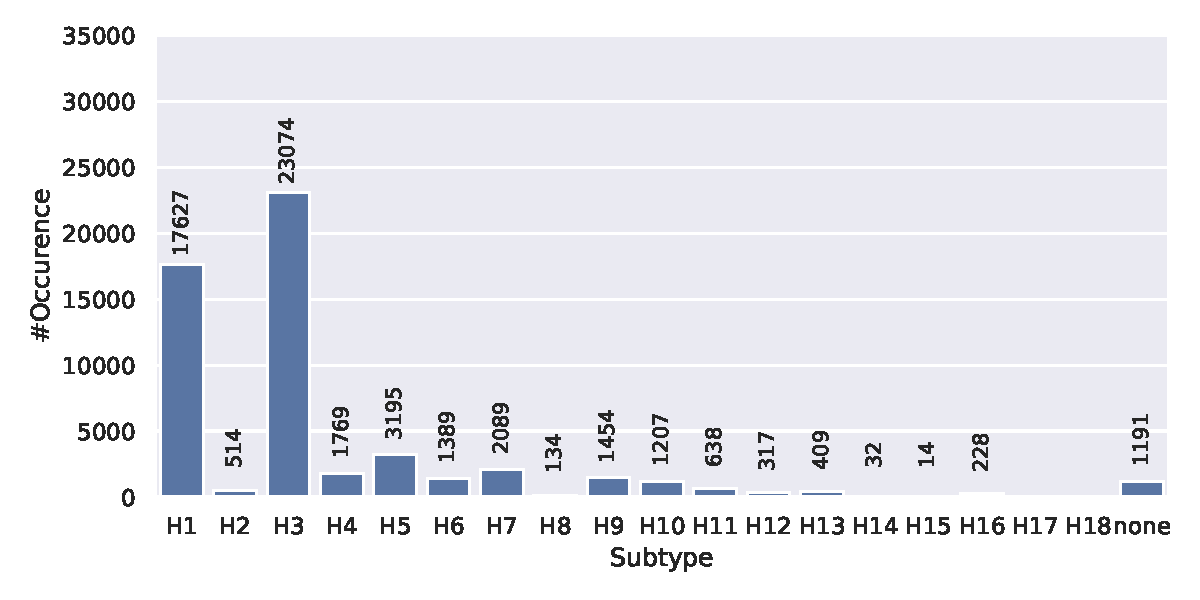
\includegraphics[width=\dimexpr\textwidth-2\fboxsep-2\fboxrule,fbox]{PCA/Data_Overview_Segment_4_H.pdf}
    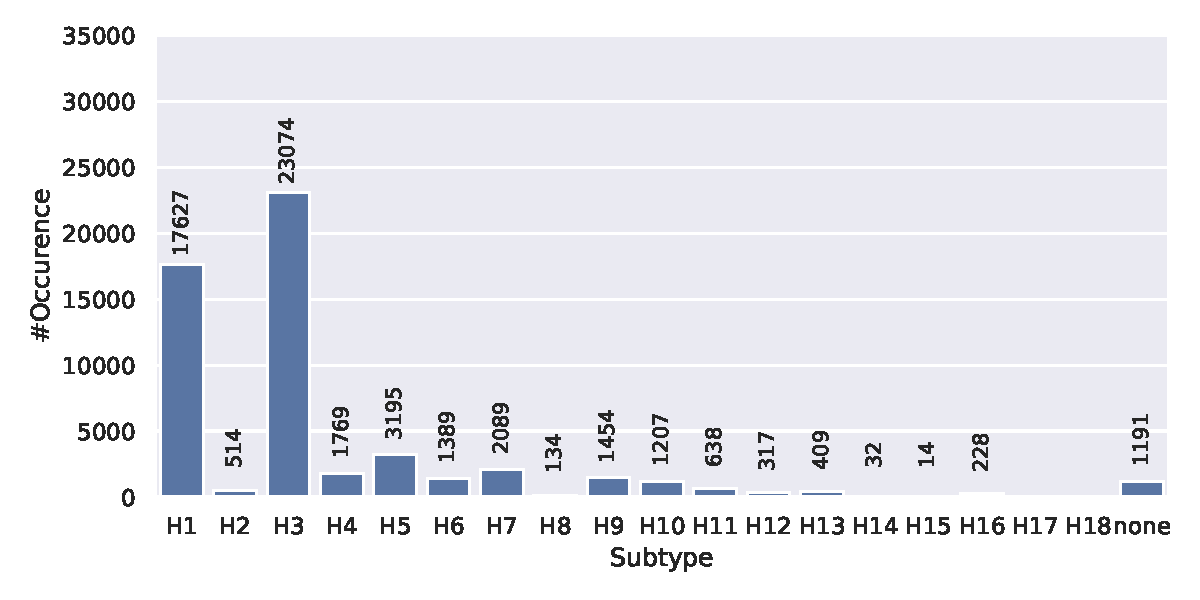
\includegraphics[width=\textwidth]{PCA/Data_Overview_Segment_4_H.pdf}
    \caption[Segment 4 \Acrlong{HA} Antigen Subtype Frequency]{\textbf{Segment 4 \Acrlong{HA} Antigen Subtype Frequency.} .}
    \label{fig:Frequency_4}
\end{figure}

\begin{figure}[!hbt]
    \centering
    %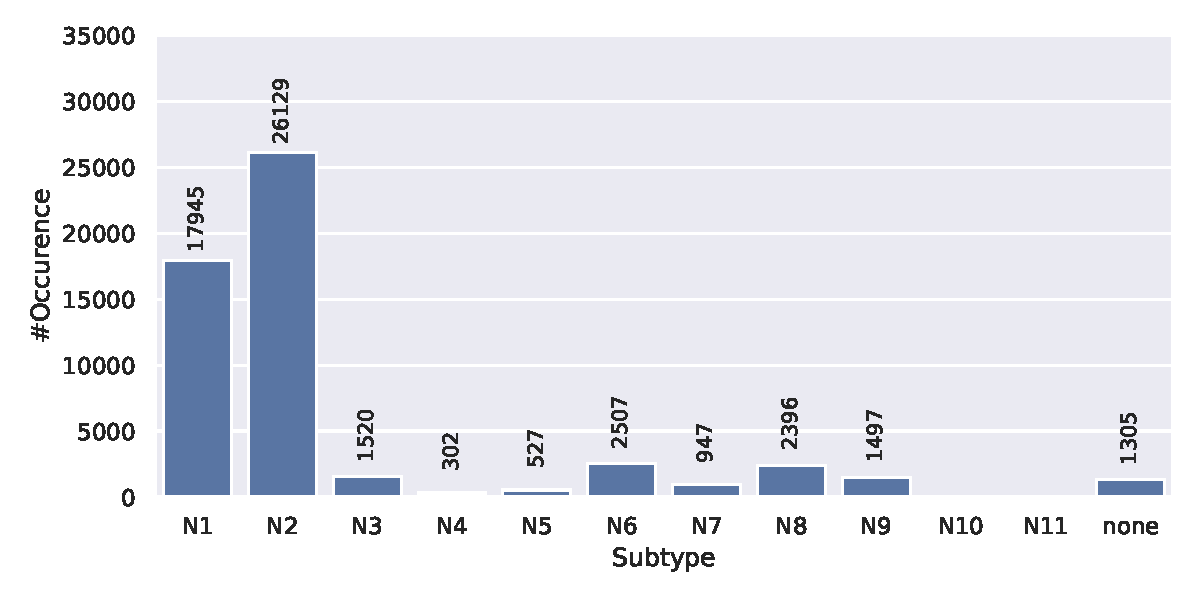
\includegraphics[width=\dimexpr\textwidth-2\fboxsep-2\fboxrule,fbox]{PCA/Data_Overview_Segment_6_N.pdf}
    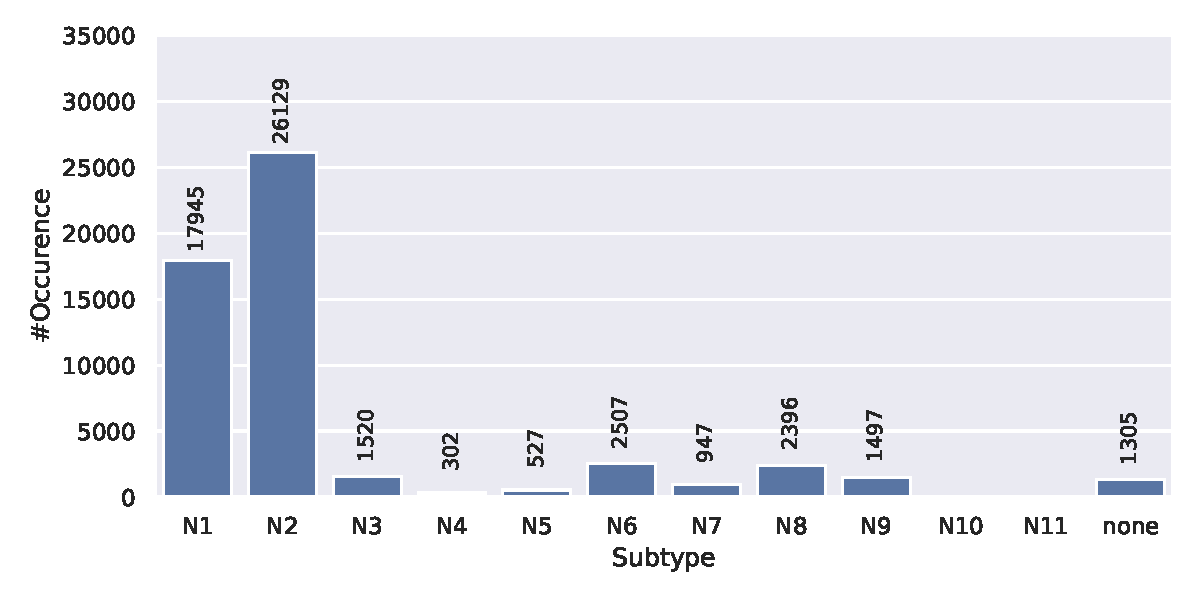
\includegraphics[width=\textwidth]{PCA/Data_Overview_Segment_6_N.pdf}
    \caption[Segment 6 \Acrlong{NA} Antigen Subtype Frequency]{\textbf{Segment 4 \Acrlong{NA} Antigen Subtype Frequency.} .}
    \label{fig:Frequency_6}
\end{figure}

\section{Clustering} \label{sec:3.1}

\blindtext

\begin{figure}
    \begin{adjustbox}{minipage=\dimexpr\textwidth-2\fboxsep-2\fboxrule,fbox}
        \begin{subfigure}[b]{0.475\textwidth}
            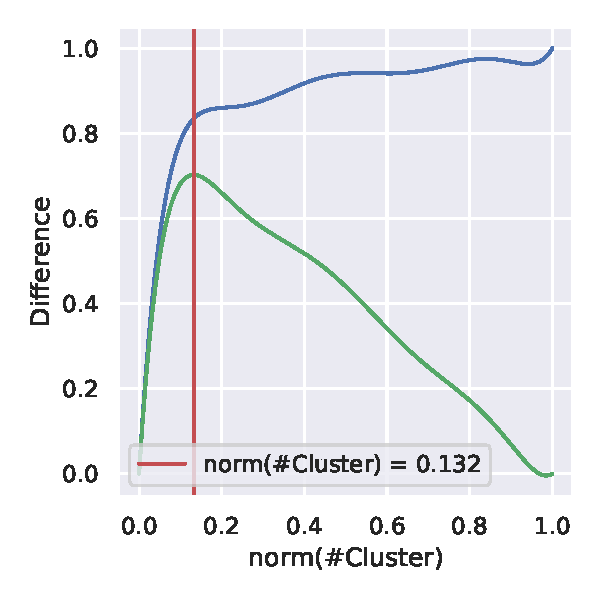
\includegraphics[width=\textwidth]{PCA/Cluster_Knee_Segment_4.pdf}
            \caption[Kneedle Algorithm]{\textbf{Kneedle Algorithm}}
            \label{fig:3.1.1a}
        \end{subfigure}
        \hfill
        \begin{subfigure}[b]{0.475\textwidth}
            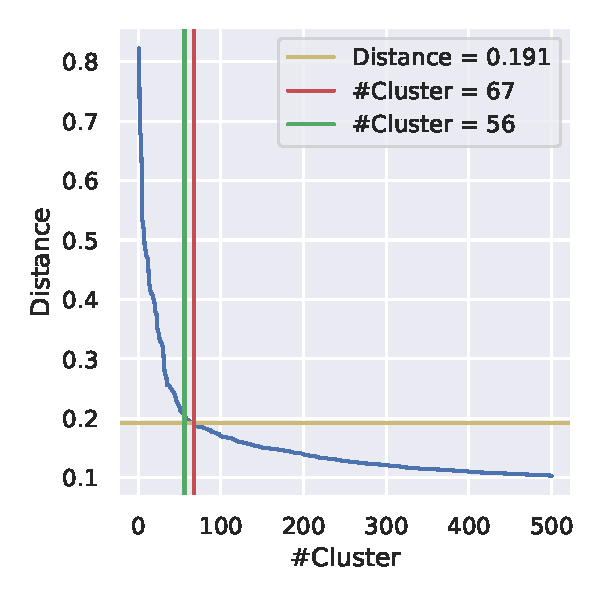
\includegraphics[width=\textwidth]{PCA/Cluster_Elbow_Knee_Segment_4.pdf}
            \caption[Kneedle Knee]{\textbf{Kneedle Knee}}
            \label{fig:3.1.1b}
        \end{subfigure}
        \vskip\baselineskip
        \begin{subfigure}[b]{0.475\textwidth}
            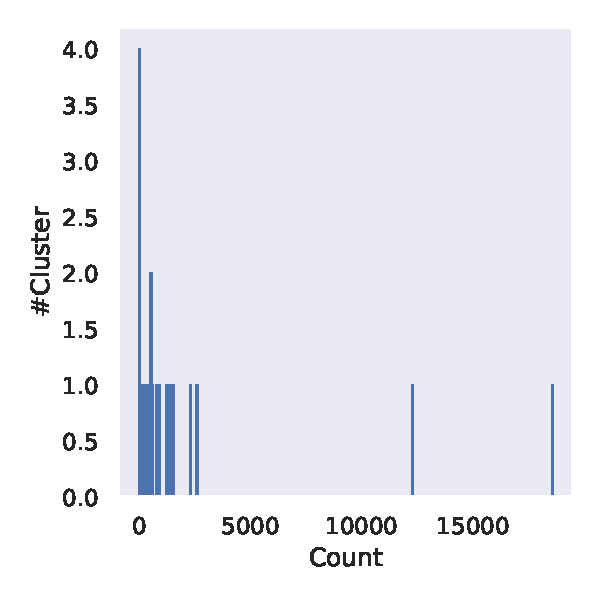
\includegraphics[width=\textwidth]{PCA/Cluster_Distribution_Segment_4.pdf}
            \caption[Cluster Distribution]{\textbf{Cluster Distribution}}
            \label{fig:3.1.1c}
        \end{subfigure}
        \hfill
        \begin{subfigure}[b]{0.475\textwidth}
            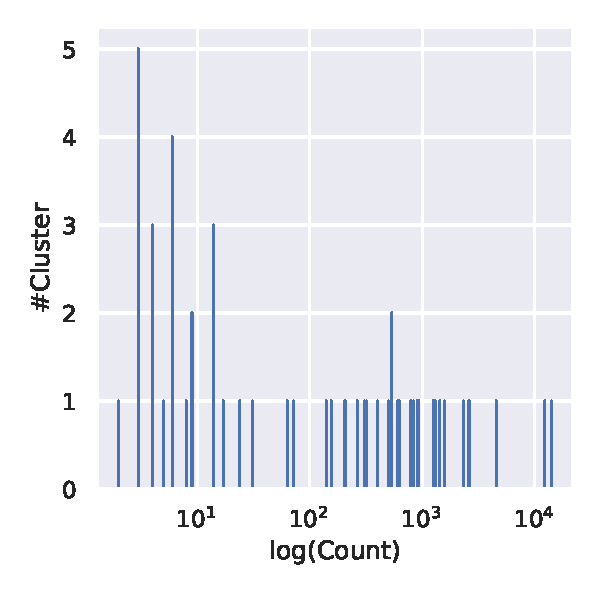
\includegraphics[width=\textwidth]{PCA/Cluster_Distribution_Log_Segment_4.pdf}
            \caption[Logarithmic Distribution]{\textbf{Logarithmic Distribution}}
            \label{fig:3.1.1d}
        \end{subfigure}
    \end{adjustbox}
    \caption[Knee based Segment 4 Clustering with PCA]{\textbf{Knee based Segment 4 Clustering with PCA.}.}
    \label{fig:3.1.1}
\end{figure}

\begin{figure}
    \begin{adjustbox}{minipage=\dimexpr\textwidth-2\fboxsep-2\fboxrule,fbox}
        \begin{subfigure}[b]{0.475\textwidth}
            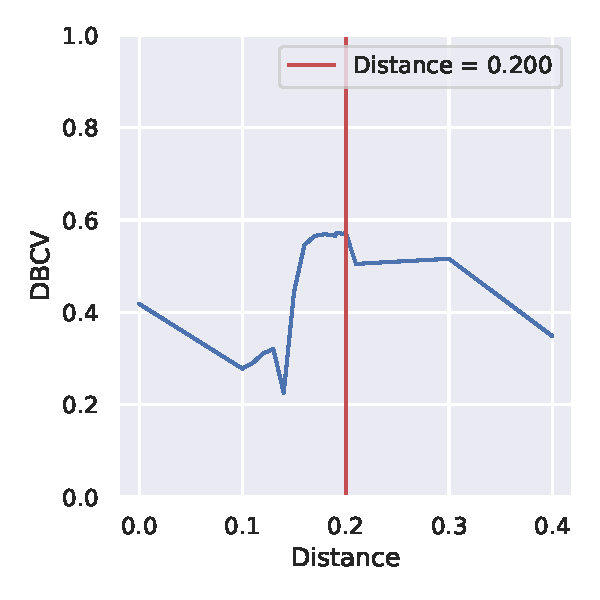
\includegraphics[width=\textwidth]{PCA/Cluster_DBCV_Segment_4.pdf}
            \caption[DBCV Exploration]{\textbf{DBCV Exploration}}
            \label{fig:3.1.2a}
        \end{subfigure}
        \hfill
        \begin{subfigure}[b]{0.475\textwidth}
            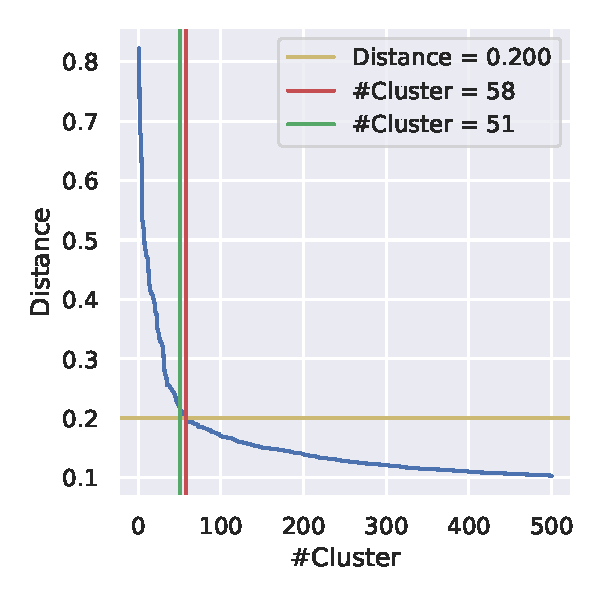
\includegraphics[width=\textwidth]{PCA/Cluster_Elbow_DBCV_Segment_4.pdf}
            \caption[DBCV Knee]{\textbf{DBCV Knee}}
            \label{fig:3.1.2b}
        \end{subfigure}
        \vskip\baselineskip
        \begin{subfigure}[b]{0.475\textwidth}
            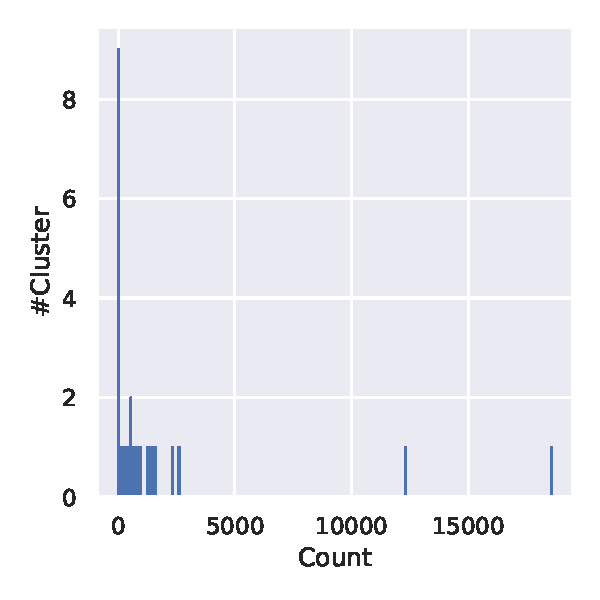
\includegraphics[width=\textwidth]{PCA/Cluster_Distribution_Segment_4_alternative.pdf}
            \caption[Cluster Distribution]{\textbf{Cluster Distribution}}
            \label{fig:3.1.2c}
        \end{subfigure}
        \hfill
        \begin{subfigure}[b]{0.475\textwidth}
            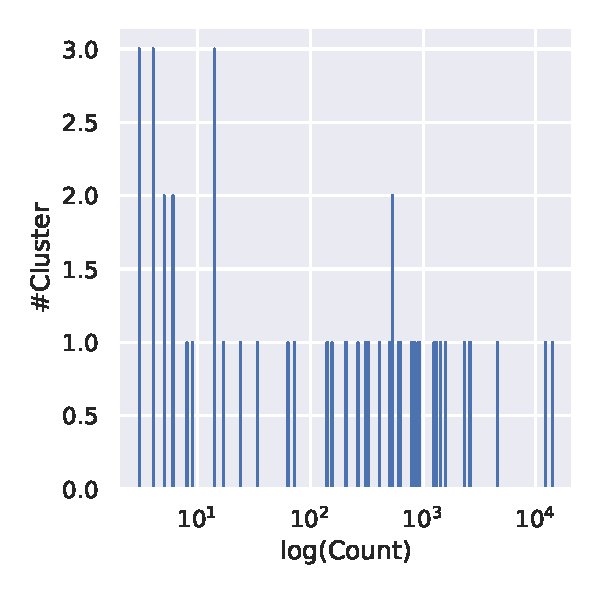
\includegraphics[width=\textwidth]{PCA/Cluster_Distribution_Log_Segment_4_alternative.pdf}
            \caption[Logarithmic Distribution]{\textbf{Logarithmic Distribution}}
            \label{fig:3.1.2d}
        \end{subfigure}
    \end{adjustbox}
    \caption[DBCV based Segment 4 Clustering with PCA]{\textbf{DBCV based Segment 4 Clustering with PCA.}.}
    \label{fig:3.1.2}
\end{figure}

\begin{figure}
    \begin{adjustbox}{minipage=\dimexpr\textwidth-2\fboxsep-2\fboxrule,fbox}
        \begin{subfigure}[b]{0.475\textwidth}
            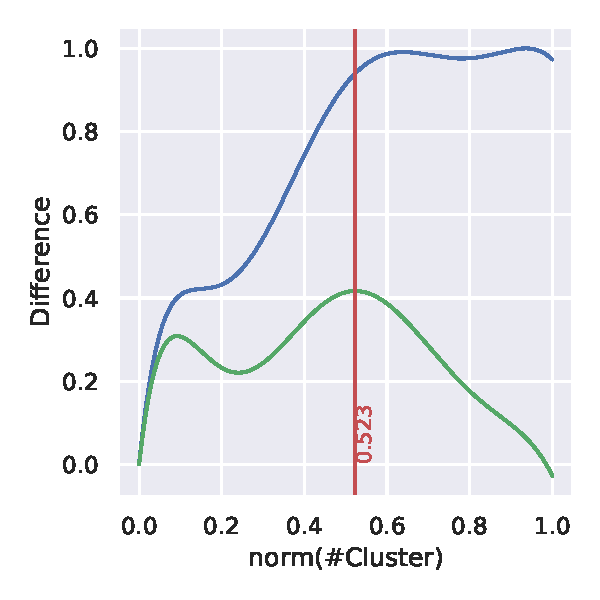
\includegraphics[width=\textwidth]{UMAP/Cluster_Knee_Segment_4.pdf}
            \caption[Kneedle Algorithm]{\textbf{Kneedle Algorithm}}
            \label{fig:3.1.3a}
        \end{subfigure}
        \hfill
        \begin{subfigure}[b]{0.475\textwidth}
            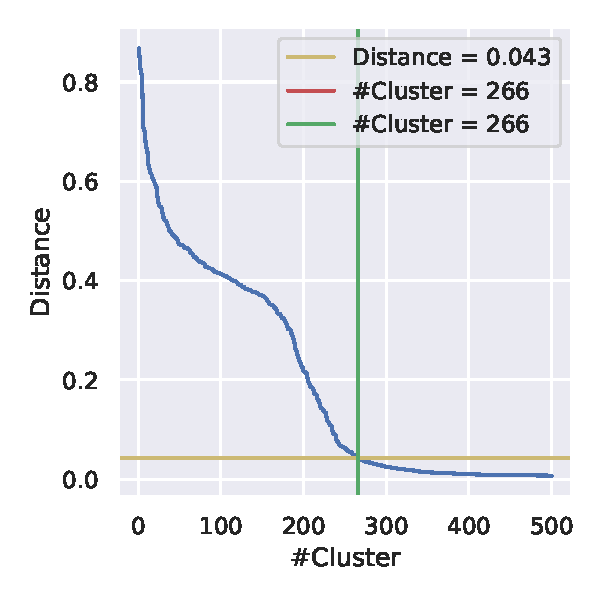
\includegraphics[width=\textwidth]{UMAP/Cluster_Elbow_Knee_Segment_4.pdf}
            \caption[Kneedle Knee]{\textbf{Kneedle Knee}}
            \label{fig:3.1.3b}
        \end{subfigure}
        \vskip\baselineskip
        \begin{subfigure}[b]{0.475\textwidth}
            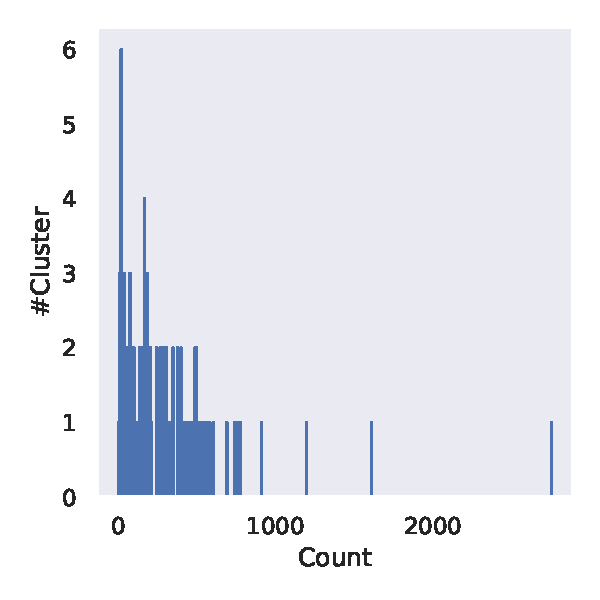
\includegraphics[width=\textwidth]{UMAP/Cluster_Distribution_Segment_4.pdf}
            \caption[Cluster Distribution]{\textbf{Cluster Distribution}}
            \label{fig:3.1.3c}
        \end{subfigure}
        \hfill
        \begin{subfigure}[b]{0.475\textwidth}
            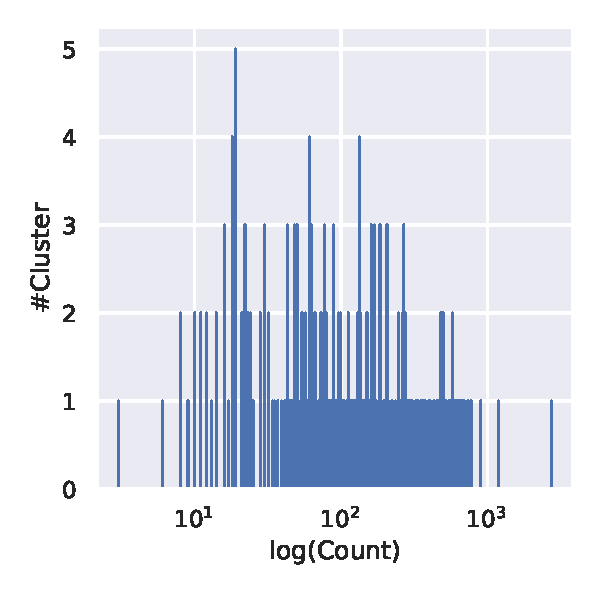
\includegraphics[width=\textwidth]{UMAP/Cluster_Distribution_Log_Segment_4.pdf}
            \caption[Logarithmic Distribution]{\textbf{Logarithmic Distribution}}
            \label{fig:3.1.3d}
        \end{subfigure}
    \end{adjustbox}
    \caption[Knee based Segment 4 Clustering with UMAP]{\textbf{Knee based Segment 4 Clustering with UMAP.}.}
    \label{fig:3.1.3}
\end{figure}

\begin{figure}
    \begin{adjustbox}{minipage=\dimexpr\textwidth-2\fboxsep-2\fboxrule,fbox}
        \begin{subfigure}[b]{0.475\textwidth}
            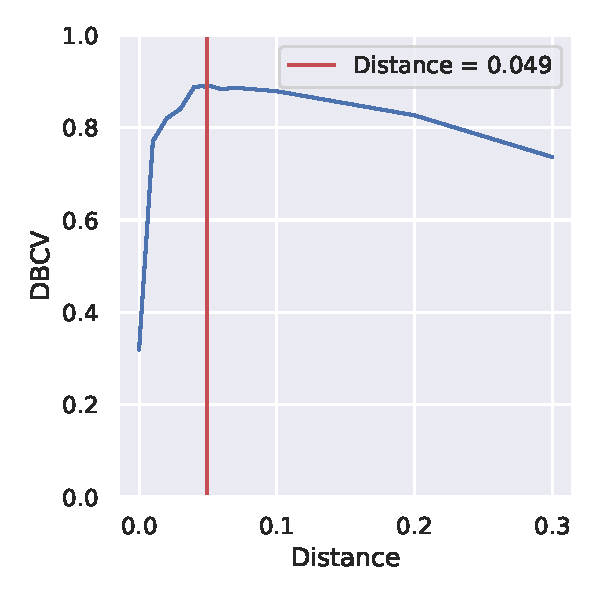
\includegraphics[width=\textwidth]{UMAP/Cluster_DBCV_Segment_4.pdf}
            \caption[DBCV Exploration]{\textbf{DBCV Exploration}}
            \label{fig:3.1.4a}
        \end{subfigure}
        \hfill
        \begin{subfigure}[b]{0.475\textwidth}
            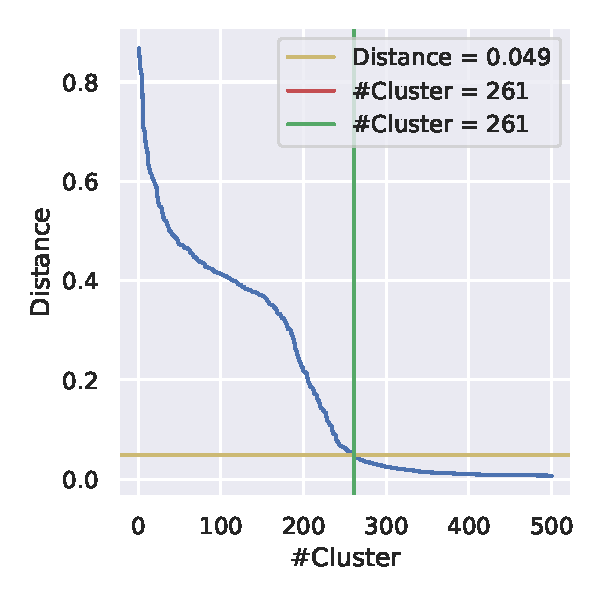
\includegraphics[width=\textwidth]{UMAP/Cluster_Elbow_DBCV_Segment_4.pdf}
            \caption[DBCV Knee]{\textbf{DBCV Knee}}
            \label{fig:3.1.4b}
        \end{subfigure}
        \vskip\baselineskip
        \begin{subfigure}[b]{0.475\textwidth}
            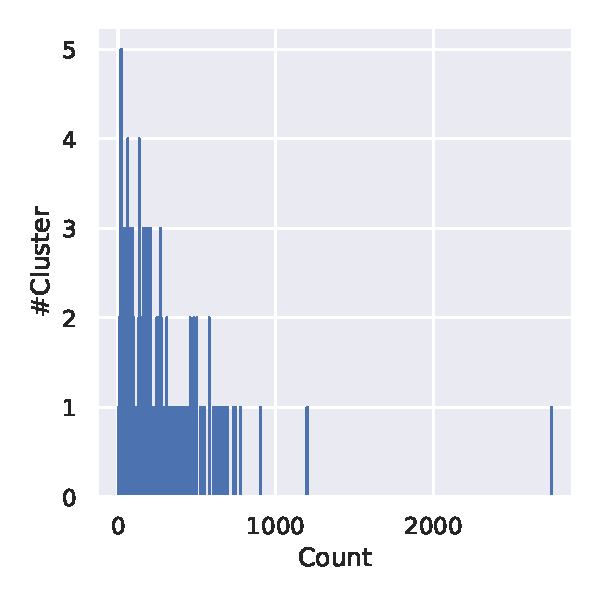
\includegraphics[width=\textwidth]{UMAP/Cluster_Distribution_Segment_4_alternative.pdf}
            \caption[Cluster Distribution]{\textbf{Cluster Distribution}}
            \label{fig:3.1.4c}
        \end{subfigure}
        \hfill
        \begin{subfigure}[b]{0.475\textwidth}
            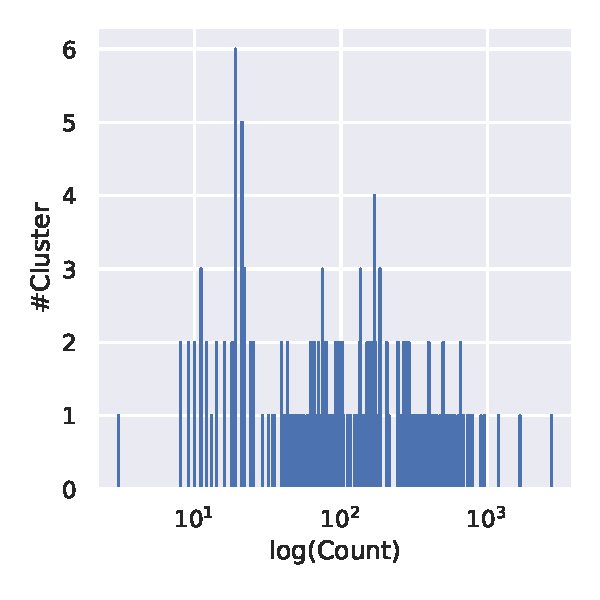
\includegraphics[width=\textwidth]{UMAP/Cluster_Distribution_Log_Segment_4_alternative.pdf}
            \caption[Logarithmic Distribution]{\textbf{Logarithmic Distribution}}
            \label{fig:3.1.4d}
        \end{subfigure}
    \end{adjustbox}
    \caption[DBCV based Segment 4 Clustering with UMAP]{\textbf{DBCV based Segment 4 Clustering with UMAP.}.}
    \label{fig:3.1.4}
\end{figure}

\begin{table}[!hbt]
    \caption[Knee based Clustering with PCA]{\textbf{Knee based Clustering with PCA.}.}
    \label{tab:3.1.1}
    \pgfplotstabletypeset[
        every head row/.style={
            before row={
                \toprule
                & \multicolumn{3}{l}{\textbf{Cluster}} &  & \multicolumn{2}{l}{\textbf{mixed}} &\\
                \cmidrule(lr){2-4}\cmidrule(lr){6-7}
            },
            after row={
                \midrule
            },
        },
        every last row/.style={
            after row={
                %... & ... & ... & ... & ... & ... & ... & ...\\
                \bottomrule
            },
        },
        begin table=\begin{tabular*}{\textwidth},
        end table=\end{tabular*},
        columns={0,1,2,3,4,5,6,7},
        columns/0/.style={multicolumn names=l,column name=\textbf{Segment}, column type=@{\extracolsep{\fill} }r},
        columns/1/.style={multicolumn names=l,column name=\textbf{\#Final}, column type=r},
        columns/2/.style={multicolumn names=l,column name=\textbf{\#Raw}, column type=r},
        columns/3/.style={multicolumn names=l,column name=\textbf{Normalized}, column type=r},
        columns/4/.style={multicolumn names=l,column name=\textbf{\#Unclustered}, column type=r},
        columns/5/.style={multicolumn names=l,column name=\textbf{H}, column type=r},
        columns/6/.style={multicolumn names=l,column name=\textbf{N}, column type=r},
        columns/7/.style={multicolumn names=l,column name=\textbf{Distance}, column type=r},
    ]
    {PCA/information.csv}
\end{table}

\begin{table}[!hbt]
    \caption[DBCV based Clustering with PCA]{\textbf{DBCV based Clustering with PCA.}.}
    \label{tab:3.1.2}
    \pgfplotstabletypeset[
        every head row/.style={
            before row={
                \toprule
                & \multicolumn{2}{l}{\textbf{Cluster}} &  & \multicolumn{2}{l}{\textbf{mixed}} & &\\
                \cmidrule(lr){2-3}\cmidrule(lr){5-6}
            },
            after row={
                \midrule
            },
        },
        every last row/.style={
            after row={
                %... & ... & ... & ... & ... & ... & ... & ...\\
                \bottomrule
            },
        },
        begin table=\begin{tabular*}{\textwidth},
        end table=\end{tabular*},
        columns={0,1,2,3,4,5,6,7},
        columns/0/.style={multicolumn names=l,column name=\textbf{Segment}, column type=@{\extracolsep{\fill} }r},
        columns/1/.style={multicolumn names=l,column name=\textbf{\#Final}, column type=r},
        columns/2/.style={multicolumn names=l,column name=\textbf{\#Raw}, column type=r},
        columns/3/.style={multicolumn names=l,column name=\textbf{\#Unclustered}, column type=r},
        columns/4/.style={multicolumn names=l,column name=\textbf{H}, column type=r},
        columns/5/.style={multicolumn names=l,column name=\textbf{N}, column type=r},
        columns/6/.style={multicolumn names=l,column name=\textbf{Distance}, column type=r},
        columns/7/.style={multicolumn names=l,column name=\textbf{DBCV}, column type=r},
    ]
    {PCA/information_alt.csv}
\end{table}

\begin{table}[!hbt]
    \caption[Knee based Clustering with UMAP]{\textbf{Knee based Clustering with UMAP.}.}
    \label{tab:3.1.3}
    \pgfplotstabletypeset[
        every head row/.style={
            before row={
                \toprule
                & \multicolumn{3}{l}{\textbf{Cluster}} &  & \multicolumn{2}{l}{\textbf{mixed}} &\\
                \cmidrule(lr){2-4}\cmidrule(lr){6-7}
            },
            after row={
                \midrule
            },
        },
        every last row/.style={
            after row={
                %... & ... & ... & ... & ... & ... & ... & ...\\
                \bottomrule
            },
        },
        begin table=\begin{tabular*}{\textwidth},
        end table=\end{tabular*},
        columns={0,1,2,3,4,5,6,7},
        columns/0/.style={multicolumn names=l,column name=\textbf{Segment}, column type=@{\extracolsep{\fill} }r},
        columns/1/.style={multicolumn names=l,column name=\textbf{\#Final}, column type=r},
        columns/2/.style={multicolumn names=l,column name=\textbf{\#Raw}, column type=r},
        columns/3/.style={multicolumn names=l,column name=\textbf{Normalized}, column type=r},
        columns/4/.style={multicolumn names=l,column name=\textbf{\#Unclustered}, column type=r},
        columns/5/.style={multicolumn names=l,column name=\textbf{H}, column type=r},
        columns/6/.style={multicolumn names=l,column name=\textbf{N}, column type=r},
        columns/7/.style={multicolumn names=l,column name=\textbf{Distance}, column type=r},
    ]
    {UMAP/information.csv}
\end{table}

\begin{table}[!hbt]
    \caption[DBCV based Clustering with PCA]{\textbf{DBCV based Clustering with PCA.}.}
    \label{tab:3.1.4}
    \pgfplotstabletypeset[
        every head row/.style={
            before row={
                \toprule
                & \multicolumn{2}{l}{\textbf{Cluster}} &  & \multicolumn{2}{l}{\textbf{mixed}} & &\\
                \cmidrule(lr){2-3}\cmidrule(lr){5-6}
            },
            after row={
                \midrule
            },
        },
        every last row/.style={
            after row={
                %... & ... & ... & ... & ... & ... & ... & ...\\
                \bottomrule
            },
        },
        begin table=\begin{tabular*}{\textwidth},
        end table=\end{tabular*},
        columns={0,1,2,3,4,5,6,7},
        columns/0/.style={multicolumn names=l,column name=\textbf{Segment}, column type=@{\extracolsep{\fill} }r},
        columns/1/.style={multicolumn names=l,column name=\textbf{\#Final}, column type=r},
        columns/2/.style={multicolumn names=l,column name=\textbf{\#Raw}, column type=r},
        columns/3/.style={multicolumn names=l,column name=\textbf{\#Unclustered}, column type=r},
        columns/4/.style={multicolumn names=l,column name=\textbf{H}, column type=r},
        columns/5/.style={multicolumn names=l,column name=\textbf{N}, column type=r},
        columns/6/.style={multicolumn names=l,column name=\textbf{Distance}, column type=r},
        columns/7/.style={multicolumn names=l,column name=\textbf{DBCV}, column type=r},
        %row predicate/.code={%
        %    \ifnum#1>0\relax
        %        \ifnum#1<2\relax
        %            \pgfplotstableuserowfalse
        %        \fi
        %    \fi
        %}
    ]
    {UMAP/information_alt.csv}
\end{table}

\blindtext

\begin{figure}[!hbt]

    \begin{annotatedFigure}
        {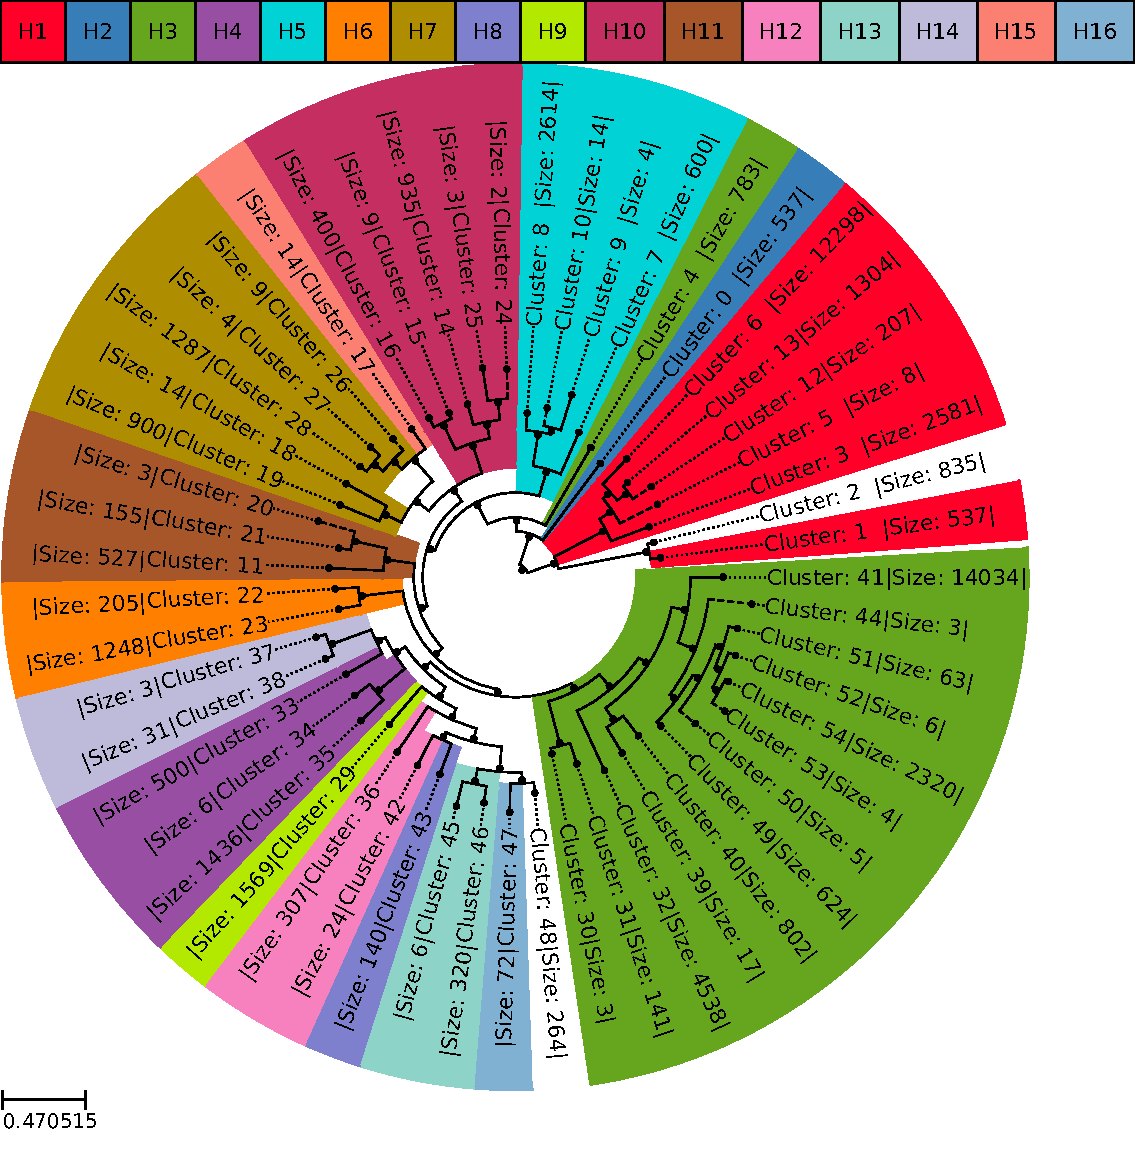
\includegraphics[width=\dimexpr\textwidth-2\fboxsep-2\fboxrule,fbox]{PCA/Clustertree_Segment_4_H_Knee.pdf}}
        \annotatedFigureBox{0.084,0.614}{0.394,0.804}{A}{0.084,0.614}%bl
    \end{annotatedFigure}
    
    \caption[Segment 4 Clustertree with PCA]{\textbf{Segment 4 Clustertree with PCA.} .}
    \label{fig:3.1.5}
\end{figure}

\begin{figure}[!hbt]
    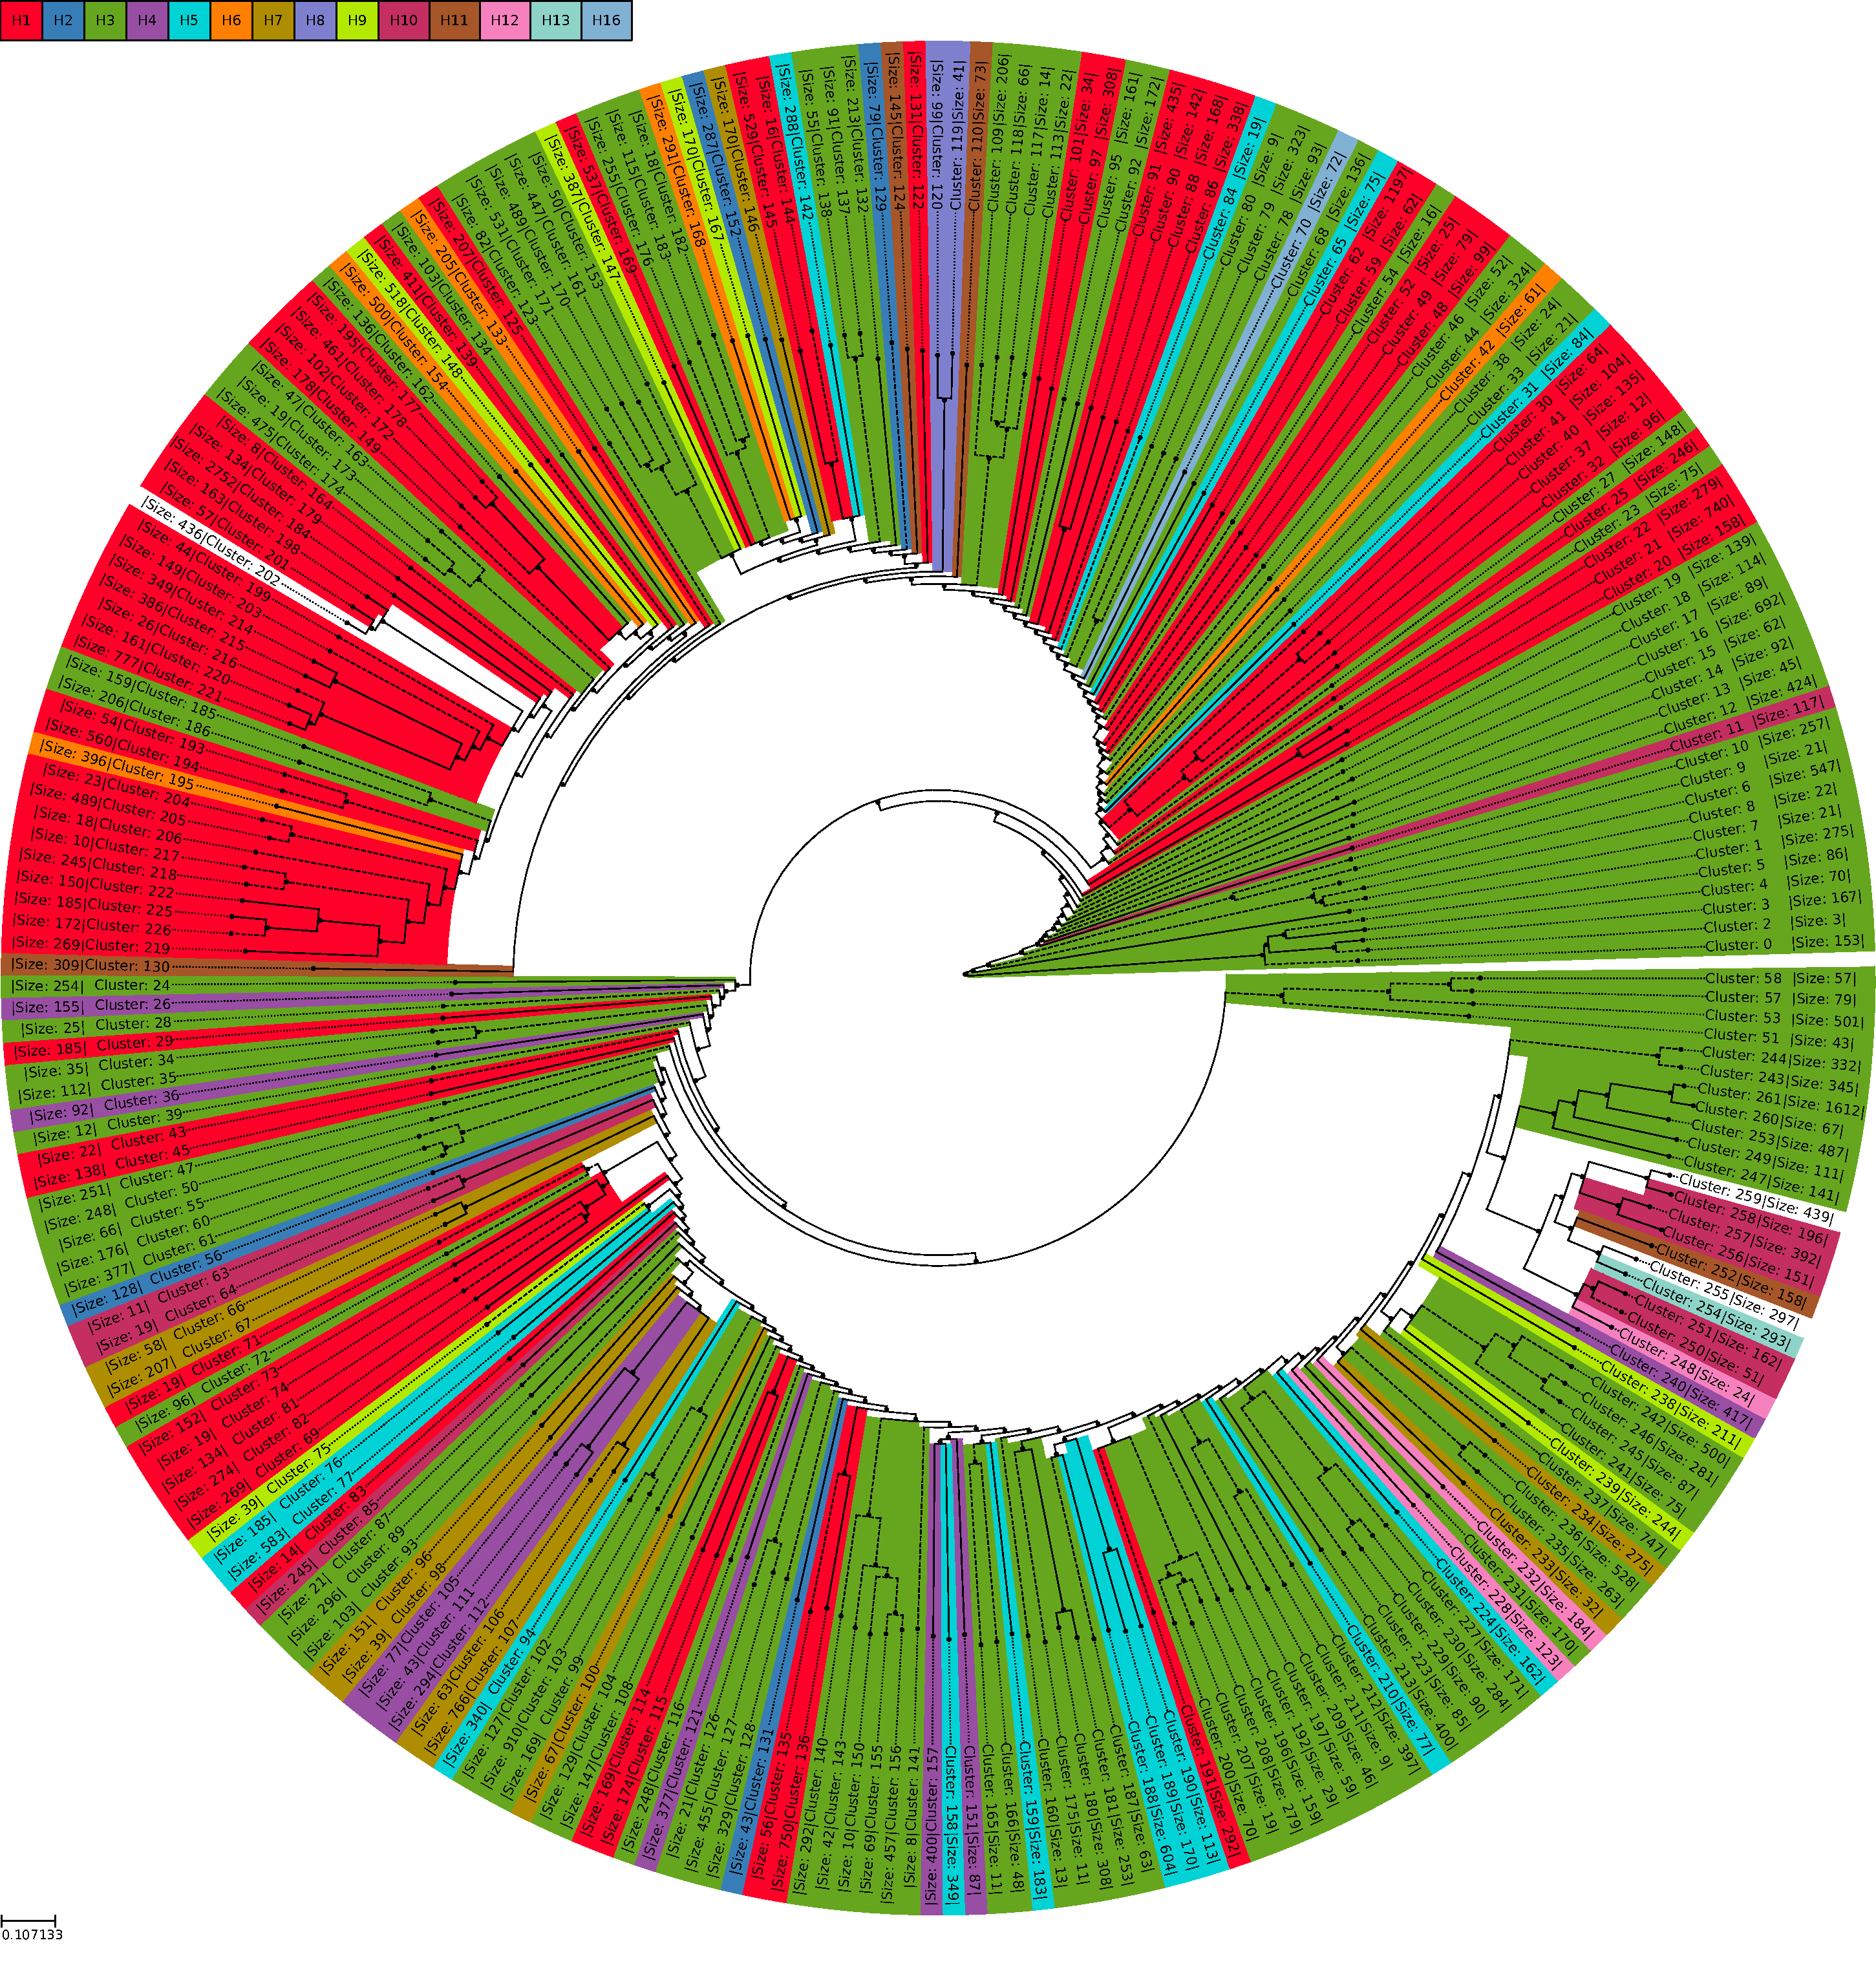
\includegraphics[width=\dimexpr\textwidth-2\fboxsep-2\fboxrule,fbox]{UMAP/Clustertree_Segment_4_H_Knee.pdf}
    \caption[Segment 4 Clustertree with UMAP]{\textbf{Segment 4 Clustertree with UMAP.} .}
    \label{fig:3.1.6}
\end{figure}

\section{Clustering Anomalies} \label{sec:Clustering_Anomalies}

\subsection{Clustering Errors}

\blindtext

\begin{table}[!hbt]
    \centering
    \caption[Anomalies in Segment 4 Cluster 2 (\Acrshort{PCA})]{\textbf{Anomalies in Segment 4 Cluster 2 (\Acrshort{PCA}).}.}
    \label{tab:PCA_Error_4_2}
    \pgfplotstabletypeset[
        every head row/.style={
            before row={
                \toprule
            },
            after row={
                \midrule
            },
        },
        every last row/.style={
            after row={
                %... & ... & ... & ... & ... & ... & ... & ...\\
                \bottomrule
            },
        },
        begin table=\begin{tabular*}{0.75\textwidth},
        end table=\end{tabular*},
        columns={0,1,2},
        columns/0/.style={string type,multicolumn names=l,column name=\textbf{Accession}, column type=@{\extracolsep{\fill}\hspace{6pt}}r},
        columns/1/.style={multicolumn names=l,column name=\textbf{H1}, column type=r},
        columns/2/.style={multicolumn names=l,column name=\textbf{H10}, column type=r},
    ]
    {PCA/error_segment_4_cluster_2_difference_head.csv}
\end{table}

\begin{table}[!hbt]
    \centering
    \caption[Anomalies in Segment 4 Cluster 48 (\Acrshort{PCA})]{\textbf{Anomalies in Segment 4 Cluster 48 (\Acrshort{PCA}).}.}
    \label{tab:PCA_Error_4_48}
    \pgfplotstabletypeset[
        every head row/.style={
            before row={
                \toprule
            },
            after row={
                \midrule
            },
        },
        every last row/.style={
            after row={
                ... & ... & ...\\
                \bottomrule
            },
        },
        begin table=\begin{tabular*}{0.75\textwidth},
        end table=\end{tabular*},
        columns={0,1,2},
        columns/0/.style={string type,multicolumn names=l,column name=\textbf{Accession}, column type=@{\extracolsep{\fill}\hspace{6pt}}r},
        columns/1/.style={multicolumn names=l,column name=\textbf{H16}, column type=r},
        columns/2/.style={multicolumn names=l,column name=\textbf{H13}, column type=r},
    ]
    {PCA/error_segment_4_cluster_48_difference_head.csv}
\end{table}

\begin{table}[!hbt]
    \centering
    \caption[Anomalies in Segment 4 Cluster 105 (\Acrshort{UMAP})]{\textbf{Anomalies in Segment 4 Cluster 105 (\Acrshort{UMAP}).}.}
    \label{tab:UMAP_Error_4_105}
    \pgfplotstabletypeset[
        every head row/.style={
            before row={
                \toprule
            },
            after row={
                \midrule
            },
        },
        every last row/.style={
            after row={
                \bottomrule
            },
        },
        begin table=\begin{tabular*}{0.75\textwidth},
        end table=\end{tabular*},
        columns={0,1,2},
        columns/0/.style={string type,multicolumn names=l,column name=\textbf{Accession}, column type=@{\extracolsep{\fill}\hspace{6pt}}r},
        columns/1/.style={multicolumn names=l,column name=\textbf{H1}, column type=r},
        columns/2/.style={multicolumn names=l,column name=\textbf{H10}, column type=r},
    ]
    {UMAP/error_segment_4_cluster_105_difference_head.csv}
\end{table}

\begin{table}[!hbt]
    \centering
    \caption[Anomalies in Segment 4 Cluster 265 (\Acrshort{UMAP})]{\textbf{Anomalies in Segment 4 Cluster 265 (\Acrshort{UMAP}).}.}
    \label{tab:UMAP_Error_4_265}
    \pgfplotstabletypeset[
        every head row/.style={
            before row={
                \toprule
            },
            after row={
                \midrule
            },
        },
        every last row/.style={
            after row={
                ... & ... & ... & ...\\
                \bottomrule
            },
        },
        begin table=\begin{tabular*}{0.75\textwidth},
        end table=\end{tabular*},
        columns={0,1,2,3},
        columns/0/.style={string type,multicolumn names=l,column name=\textbf{Accession}, column type=@{\extracolsep{\fill}\hspace{6pt}}r},
        columns/1/.style={multicolumn names=l,column name=\textbf{H7}, column type=r},
        columns/2/.style={multicolumn names=l,column name=\textbf{H10}, column type=r},
        columns/3/.style={multicolumn names=l,column name=\textbf{H12}, column type=r},
    ]
    {UMAP/error_segment_4_cluster_265_difference_head.csv}
\end{table}

\subsection{Centroid Guidetrees}

\blindtext

\begin{figure}[!hbt]
    \centering
    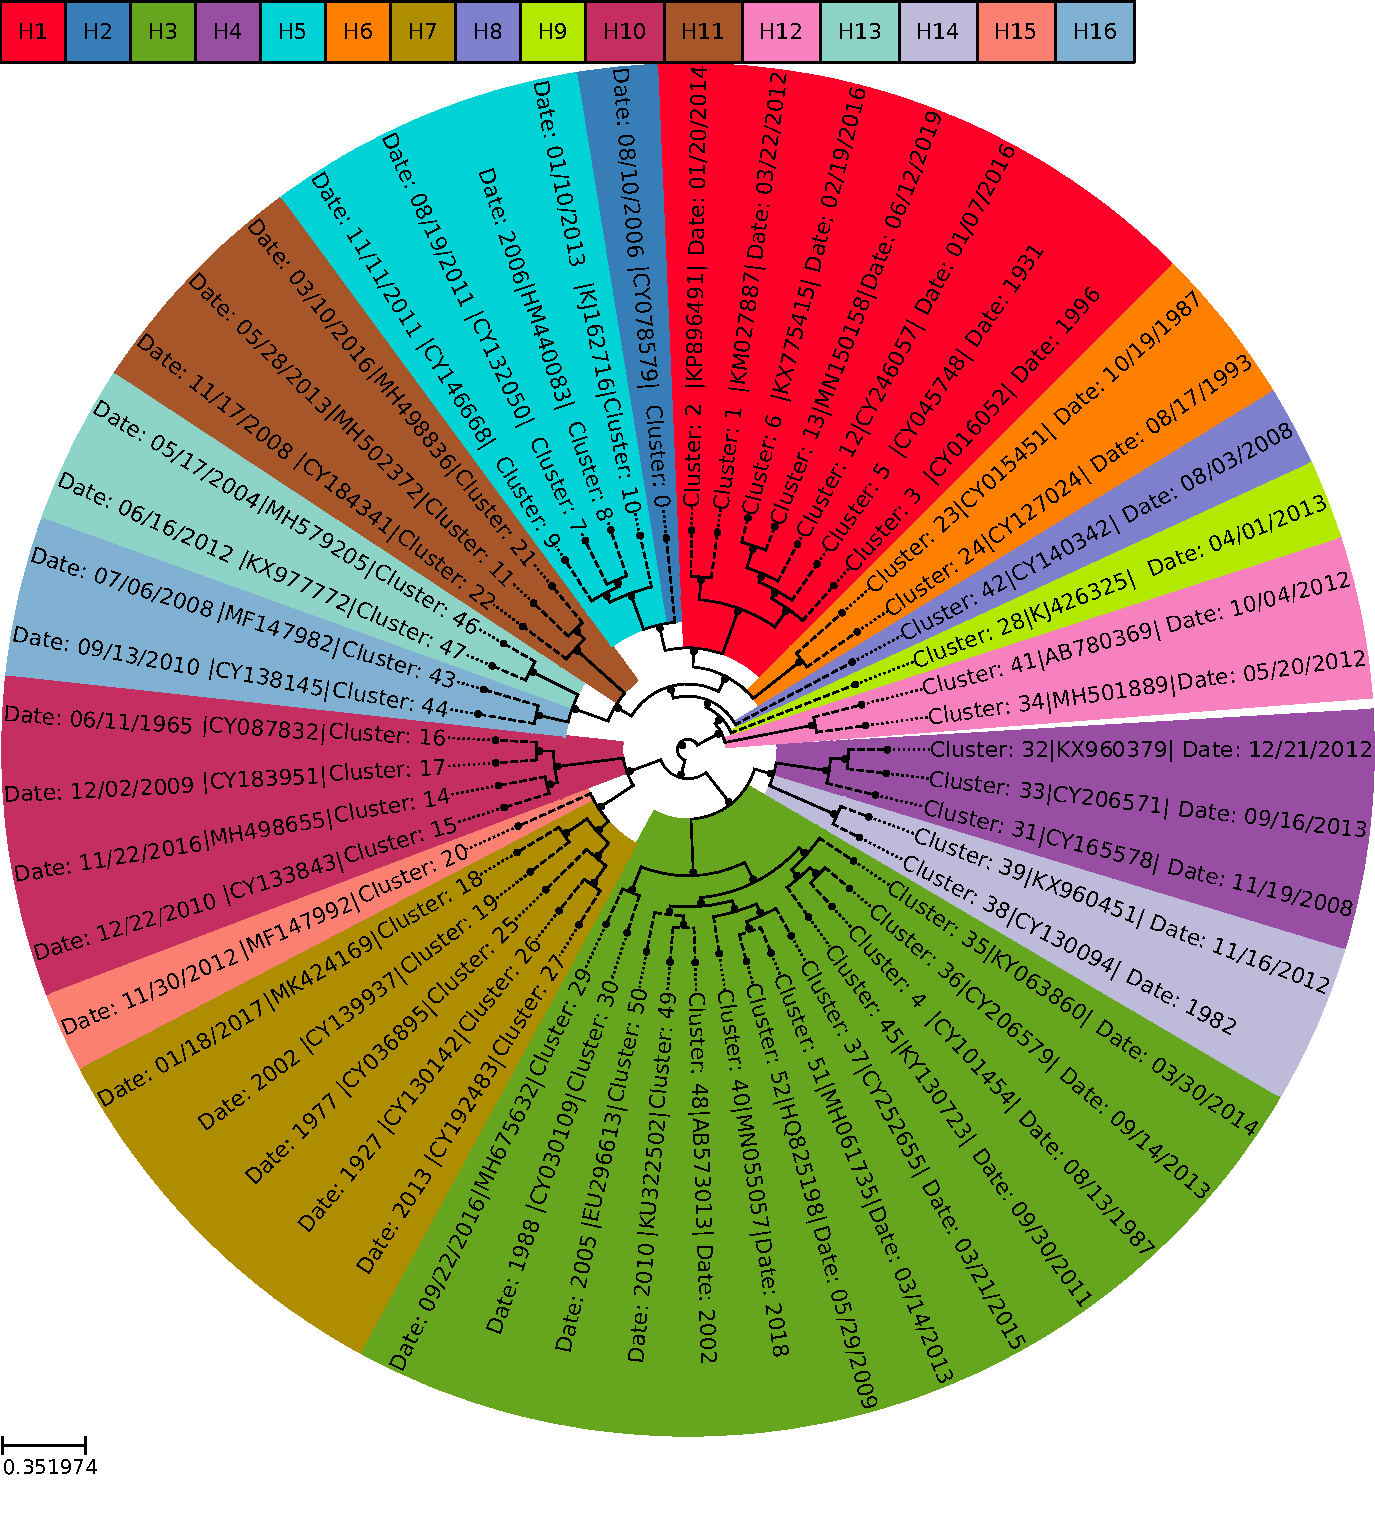
\includegraphics[width=\dimexpr\textwidth-2\fboxsep-2\fboxrule,fbox]{PCA/Guidetree_segment_4_H_Centroid.pdf}
    \caption[Knee based Segment 4 Centroid Guidetree (\Acrshort{PCA})]{\textbf{Knee based Segment 4 Centroid Guidetree (\Acrshort{PCA}).} .}
    \label{fig:PCA_Guidetree_Centroid_4}
\end{figure}

\blindtext

\begin{figure}[!hbt]
    \centering
    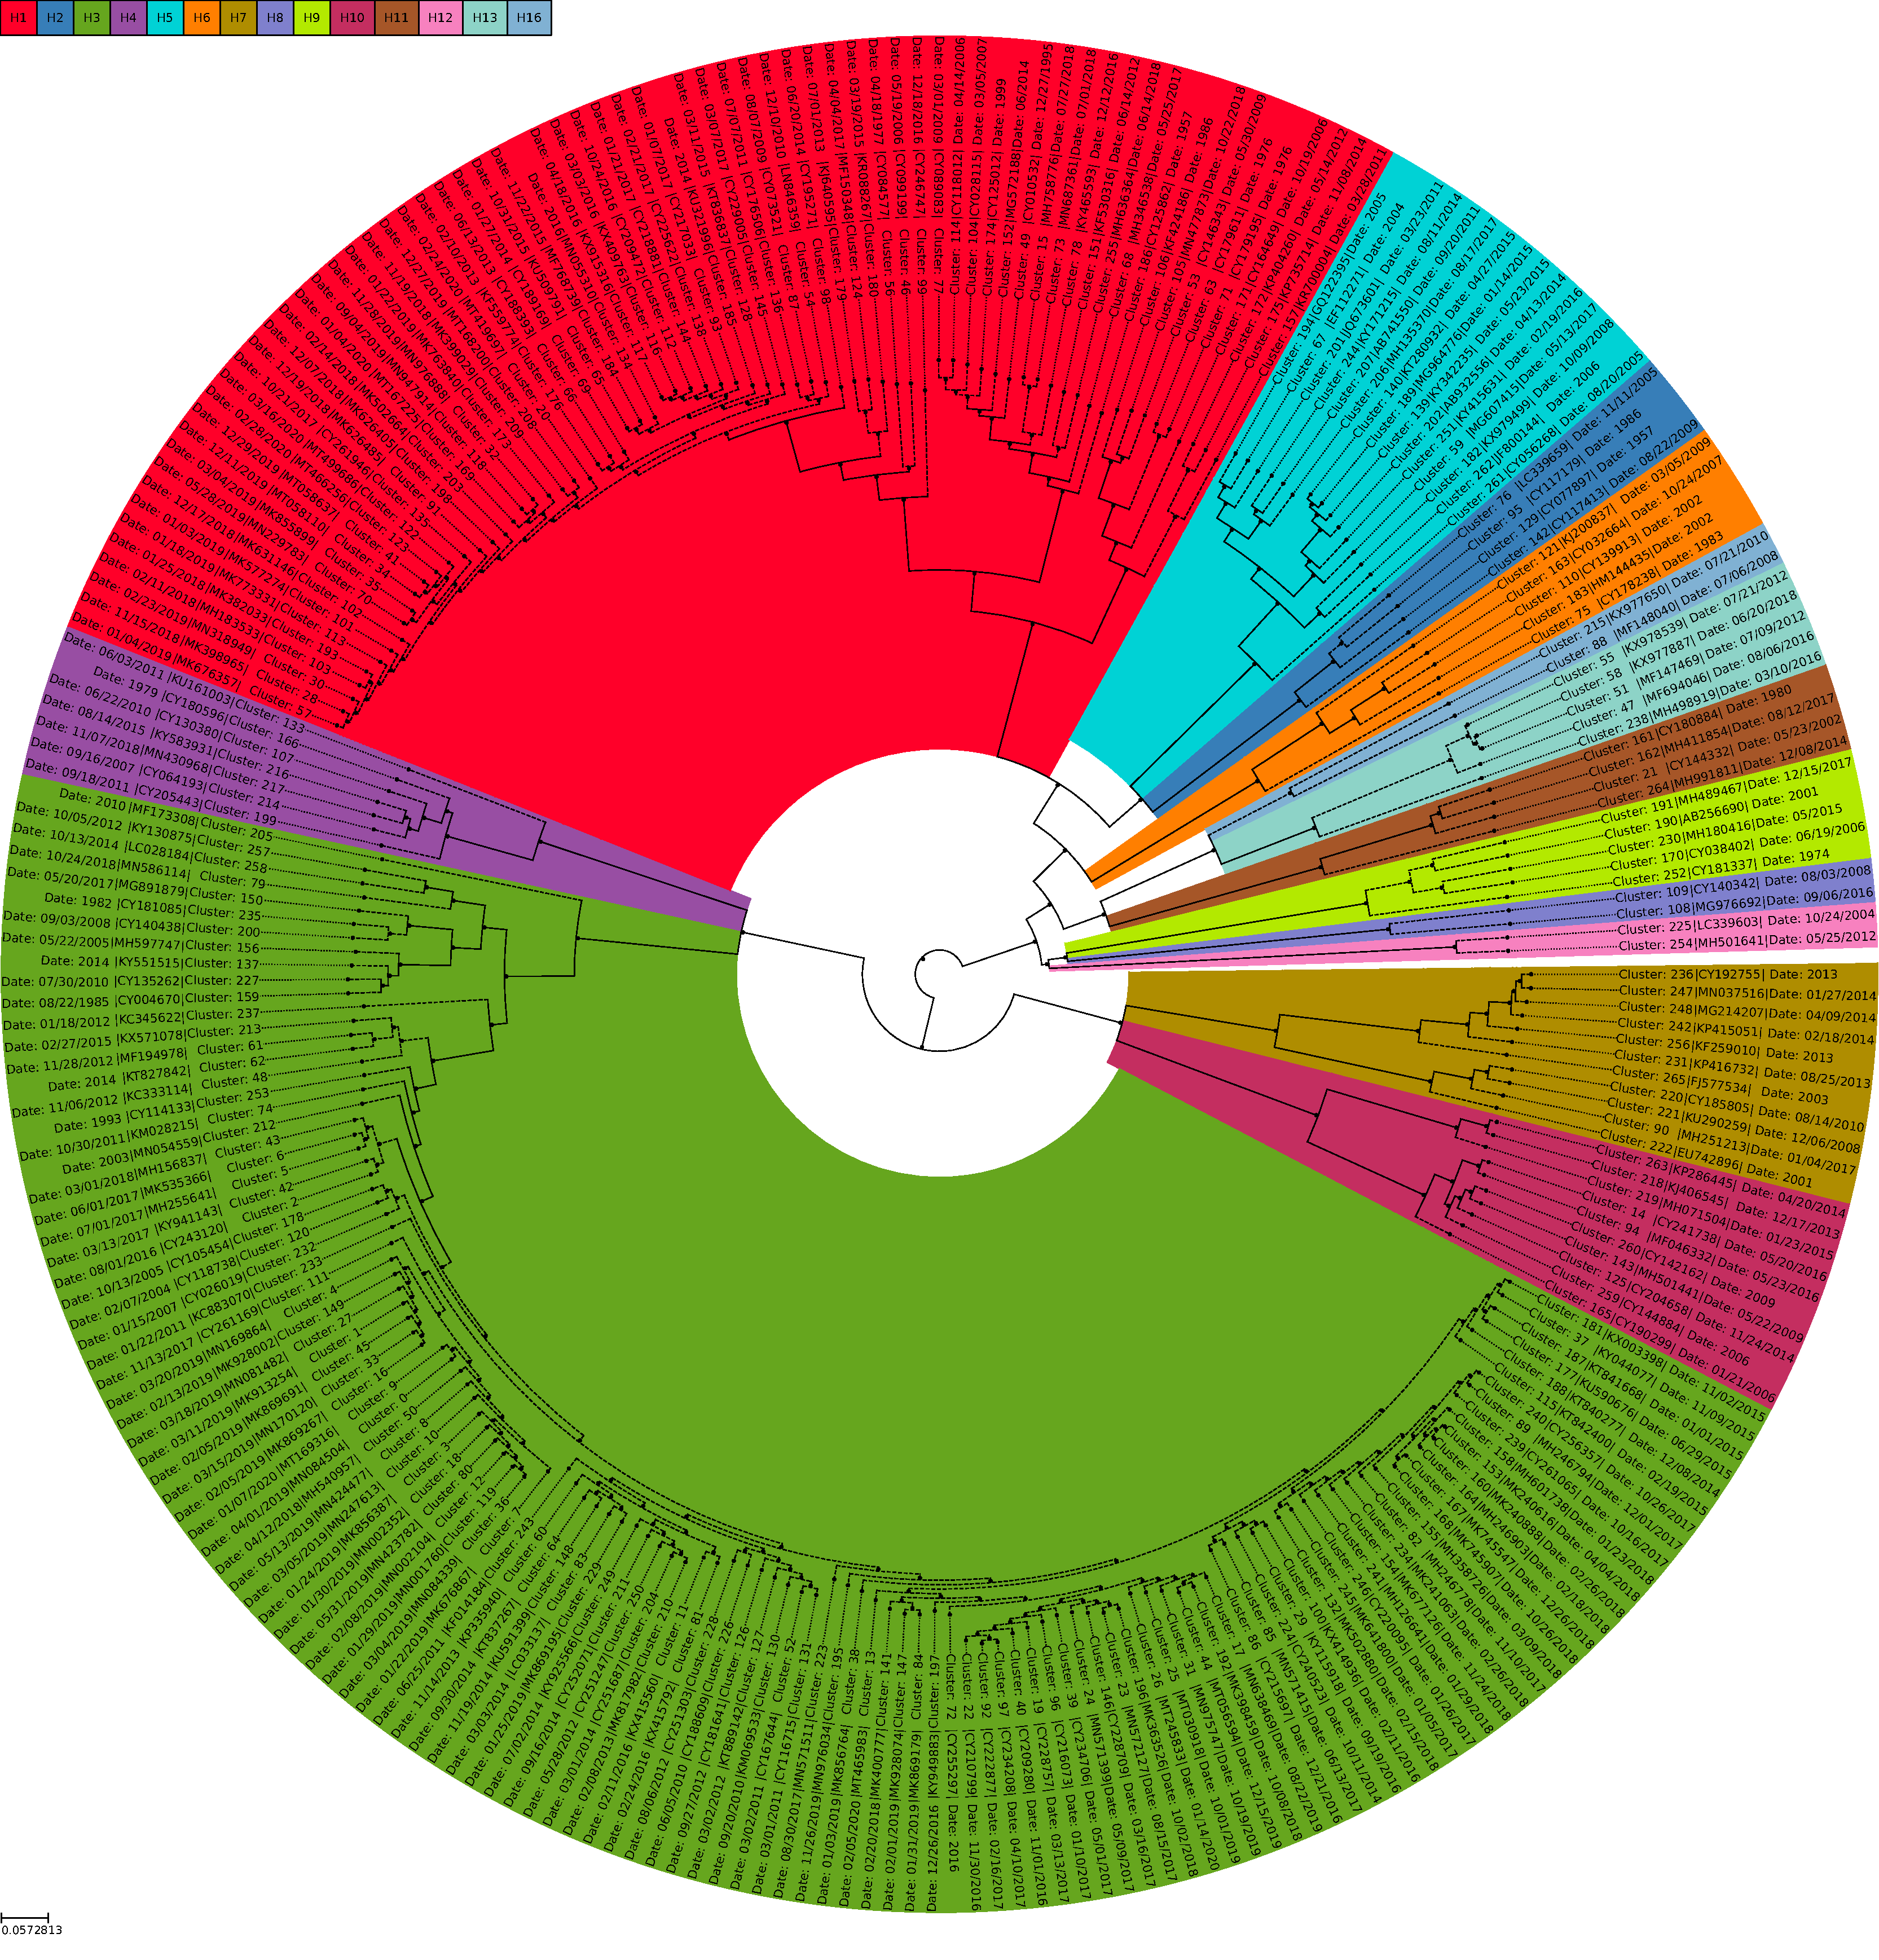
\includegraphics[width=\dimexpr\textwidth-2\fboxsep-2\fboxrule,fbox]{UMAP/Guidetree_segment_4_H_Centroid.pdf}
    \caption[Knee based Segment 4 Centroid Guidetree (\Acrshort{UMAP})]{\textbf{Knee based Segment 4 Centroid Guidetree (\Acrshort{UMAP}).} .}
    \label{fig:UMAP_Guidetree_Centroid_4}
\end{figure}

%Übergang zu cluster Comparison durch Centroid Alignment Tree -> H13/H16 Clustertree, Alignmenttree Vergleich -> Cluster H13/H16 Comparison

\section{K-mer Representation Quality} \label{sec:K_mer_Representation}

Investigation on the anomalies resulted in two persistent clustering errors (\autoref{fig:PCA_Cluster_Knee_4} \textbf{\textsf{B}} and \textbf{\textsf{D}}). To evaluate if the method is suitable for the clustering of \gls{IAV} possible error sources are discussed.

% \begin{figure}[!hbt]
%     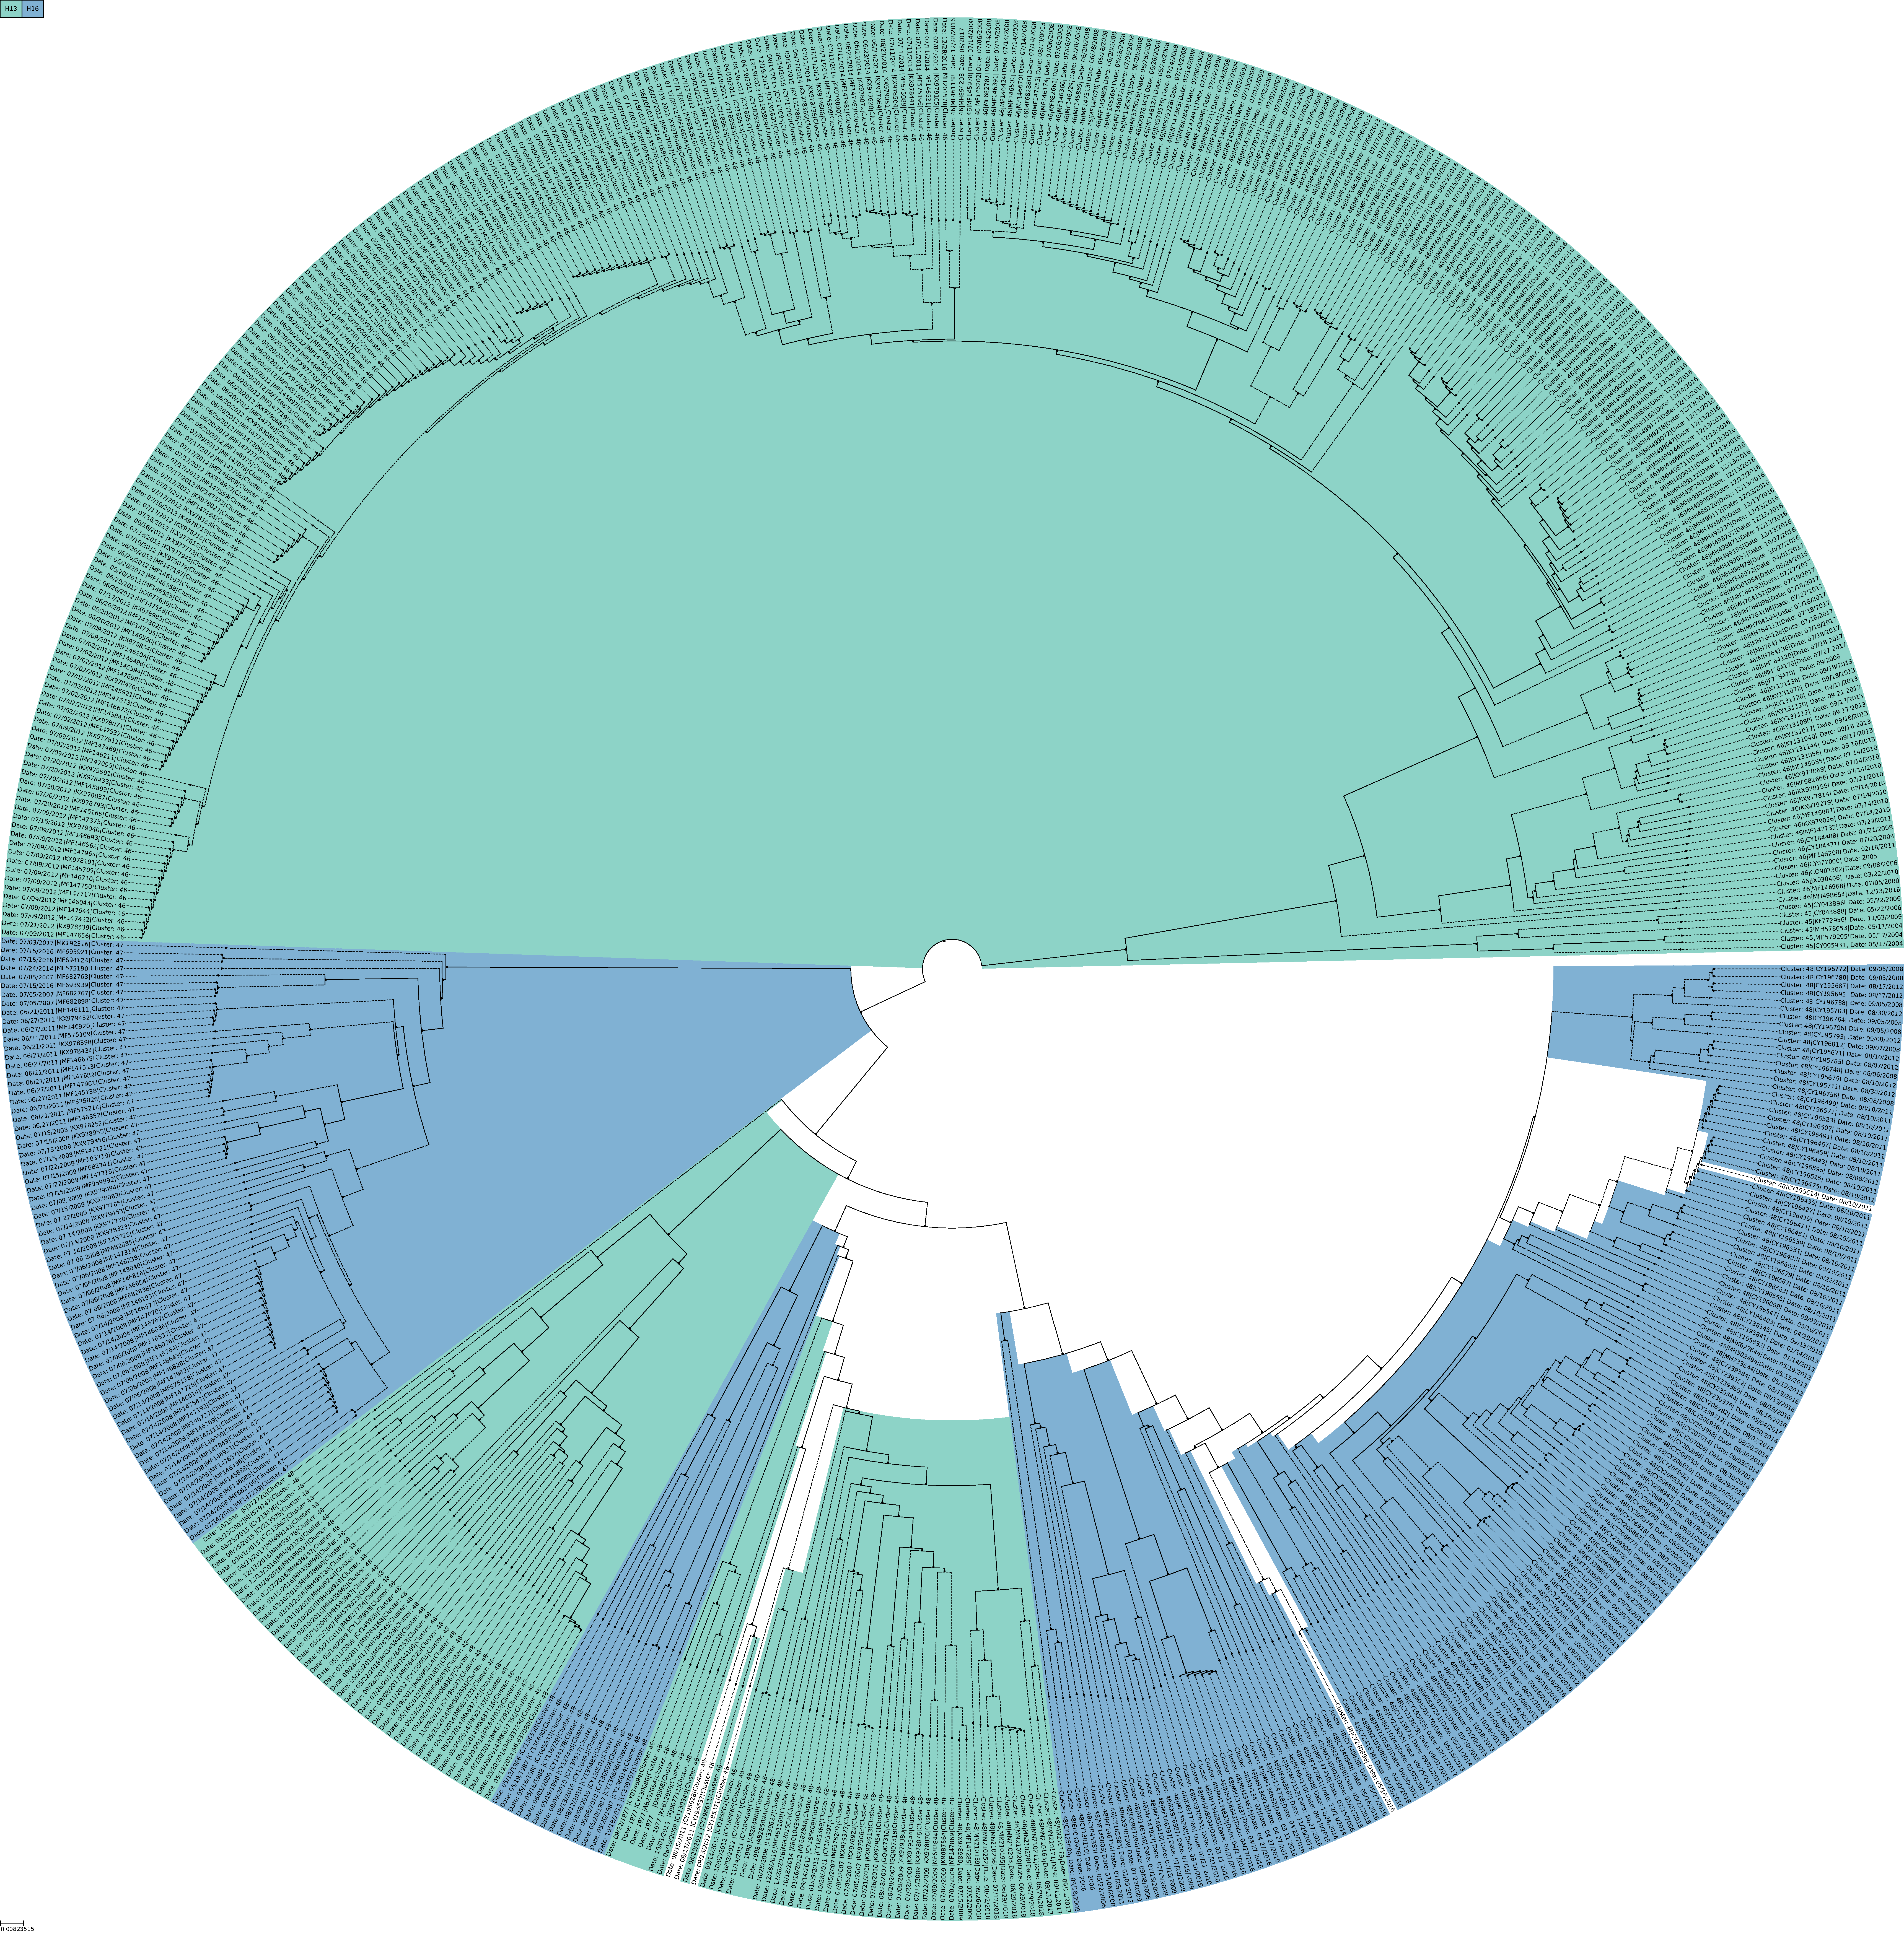
\includegraphics[width=\dimexpr\textwidth-2\fboxsep-2\fboxrule,fbox]{PCA/Clustertree_Segment_4_H_Knee_Zoom.pdf}
%     \caption[H13/H16 Simple Clustering Example with \Acrshort{PCA}]{\textbf{H13/H16 Simple Clustering Example with \Acrshort{PCA}.} .}
%     \label{fig:PCA_Clusteree_Knee_Zoom}
% \end{figure}

% \begin{figure}[!hbt]
%     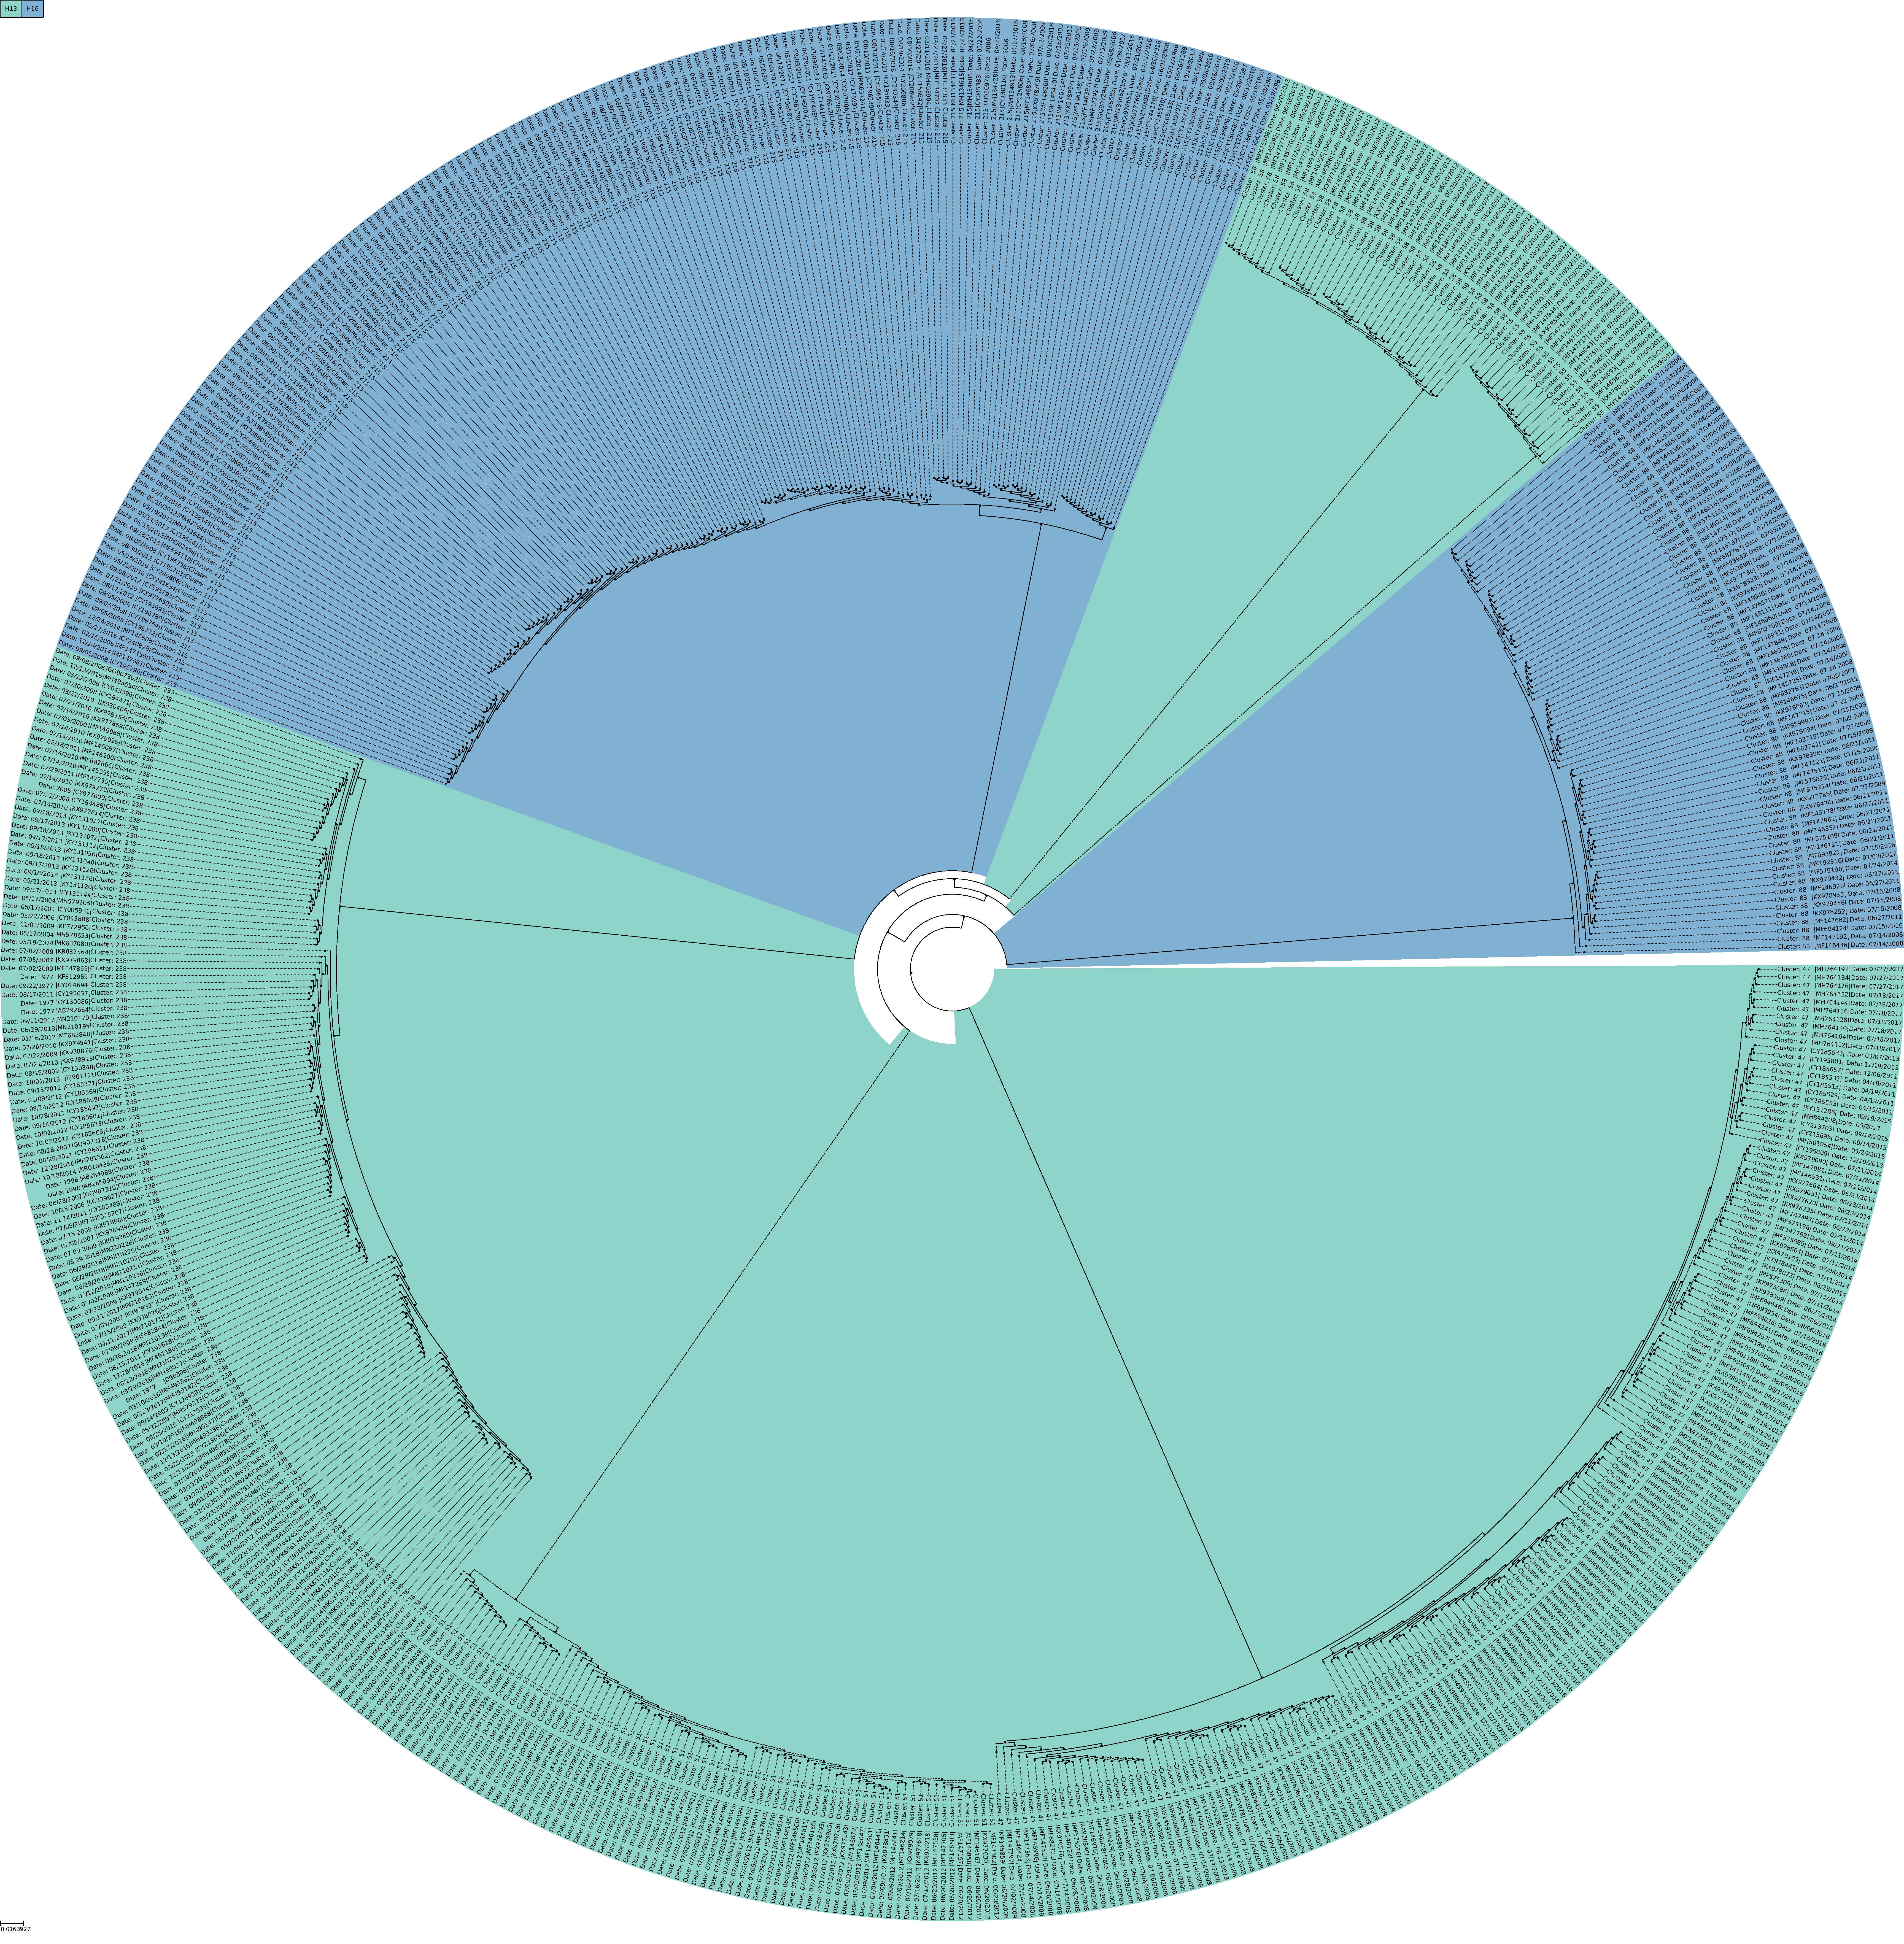
\includegraphics[width=\dimexpr\textwidth-2\fboxsep-2\fboxrule,fbox]{UMAP/Clustertree_Segment_4_H_Knee_Zoom.pdf}
%     \caption[H13/H16 Simple Clustering Example with \Acrshort{UMAP}]{\textbf{H13/H16 Simple Clustering Example with \Acrshort{UMAP}.} .}
%     \label{fig:UMAP_Clusteree_Knee_Zoom}
% \end{figure}

% \begin{figure}[!hbt]
%     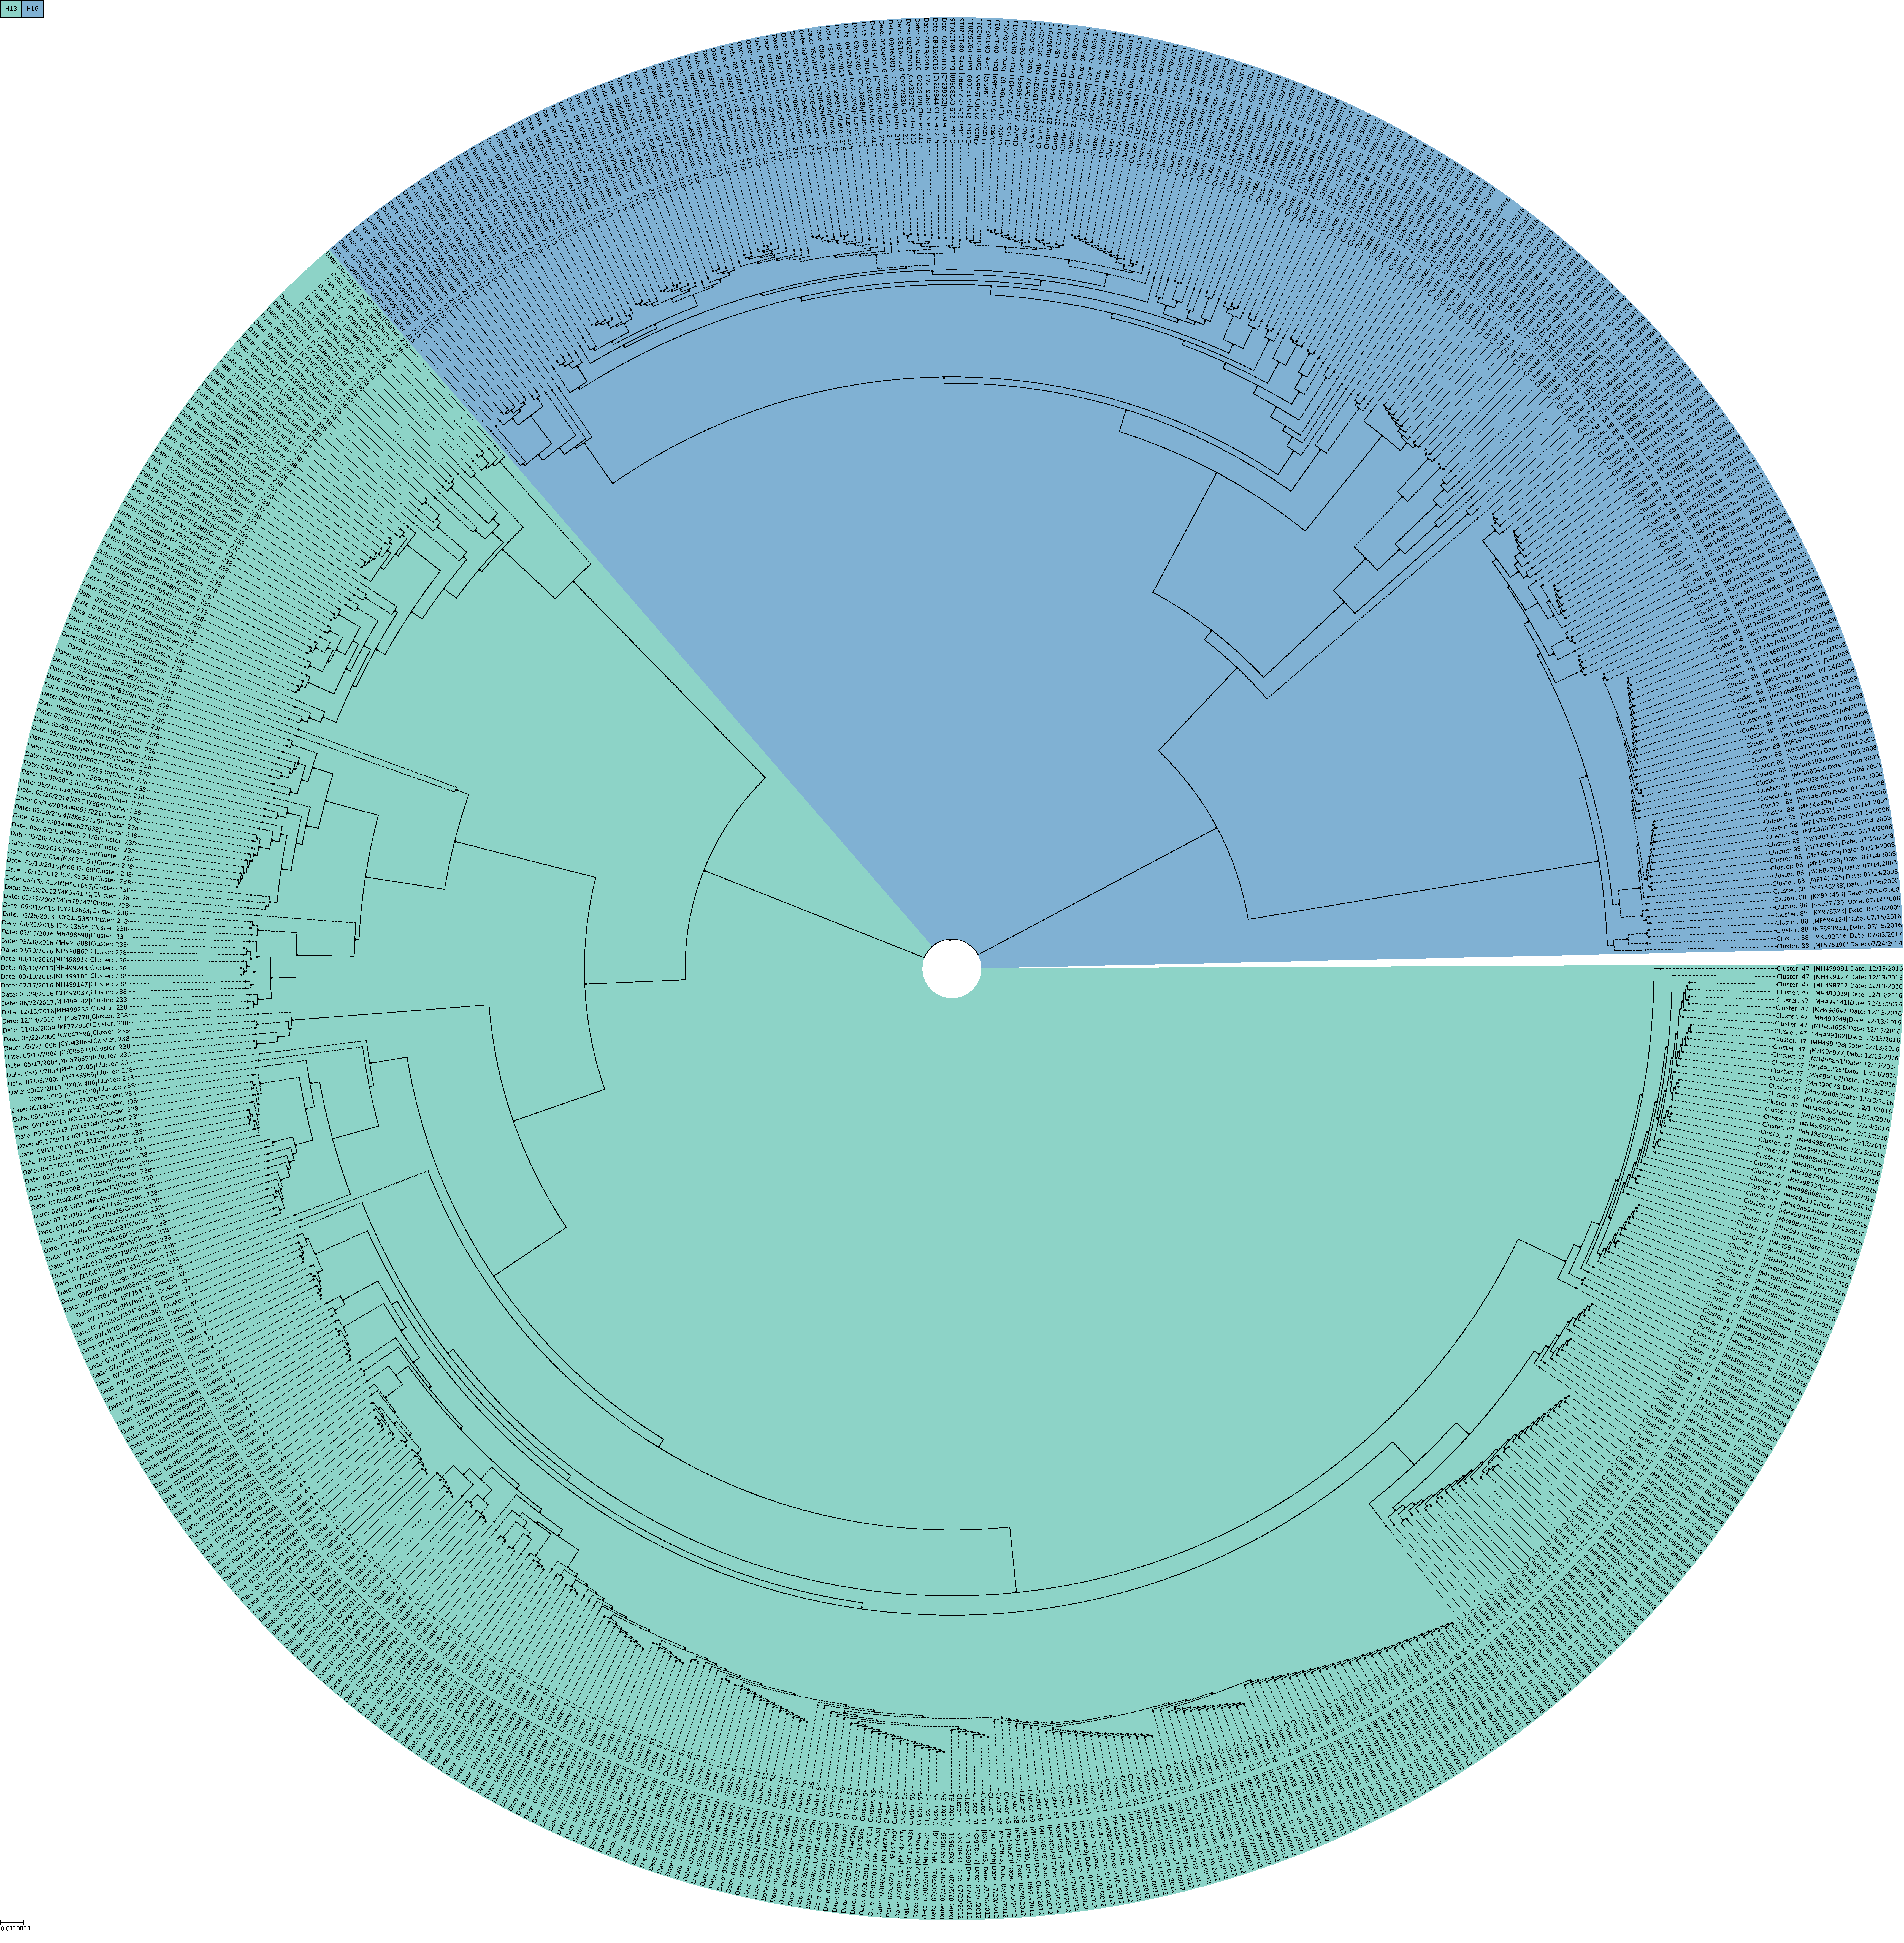
\includegraphics[width=\dimexpr\textwidth-2\fboxsep-2\fboxrule,fbox]{UMAP/Guidetree_Segment_4_H_Focus.pdf}
%     \caption[H13/H16 Simple Clustering Example with \Acrshort{MSA}]{\textbf{H13/H16 Simple Clustering Example with \Acrshort{MSA}.} .}
%     \label{fig:Guidetree_Focus}
% \end{figure}

\begin{figure}[!hbt]
    \centering
    \begin{tikzpicture}
        \node[anchor=south west,inner sep=0] (image) at (0,0) {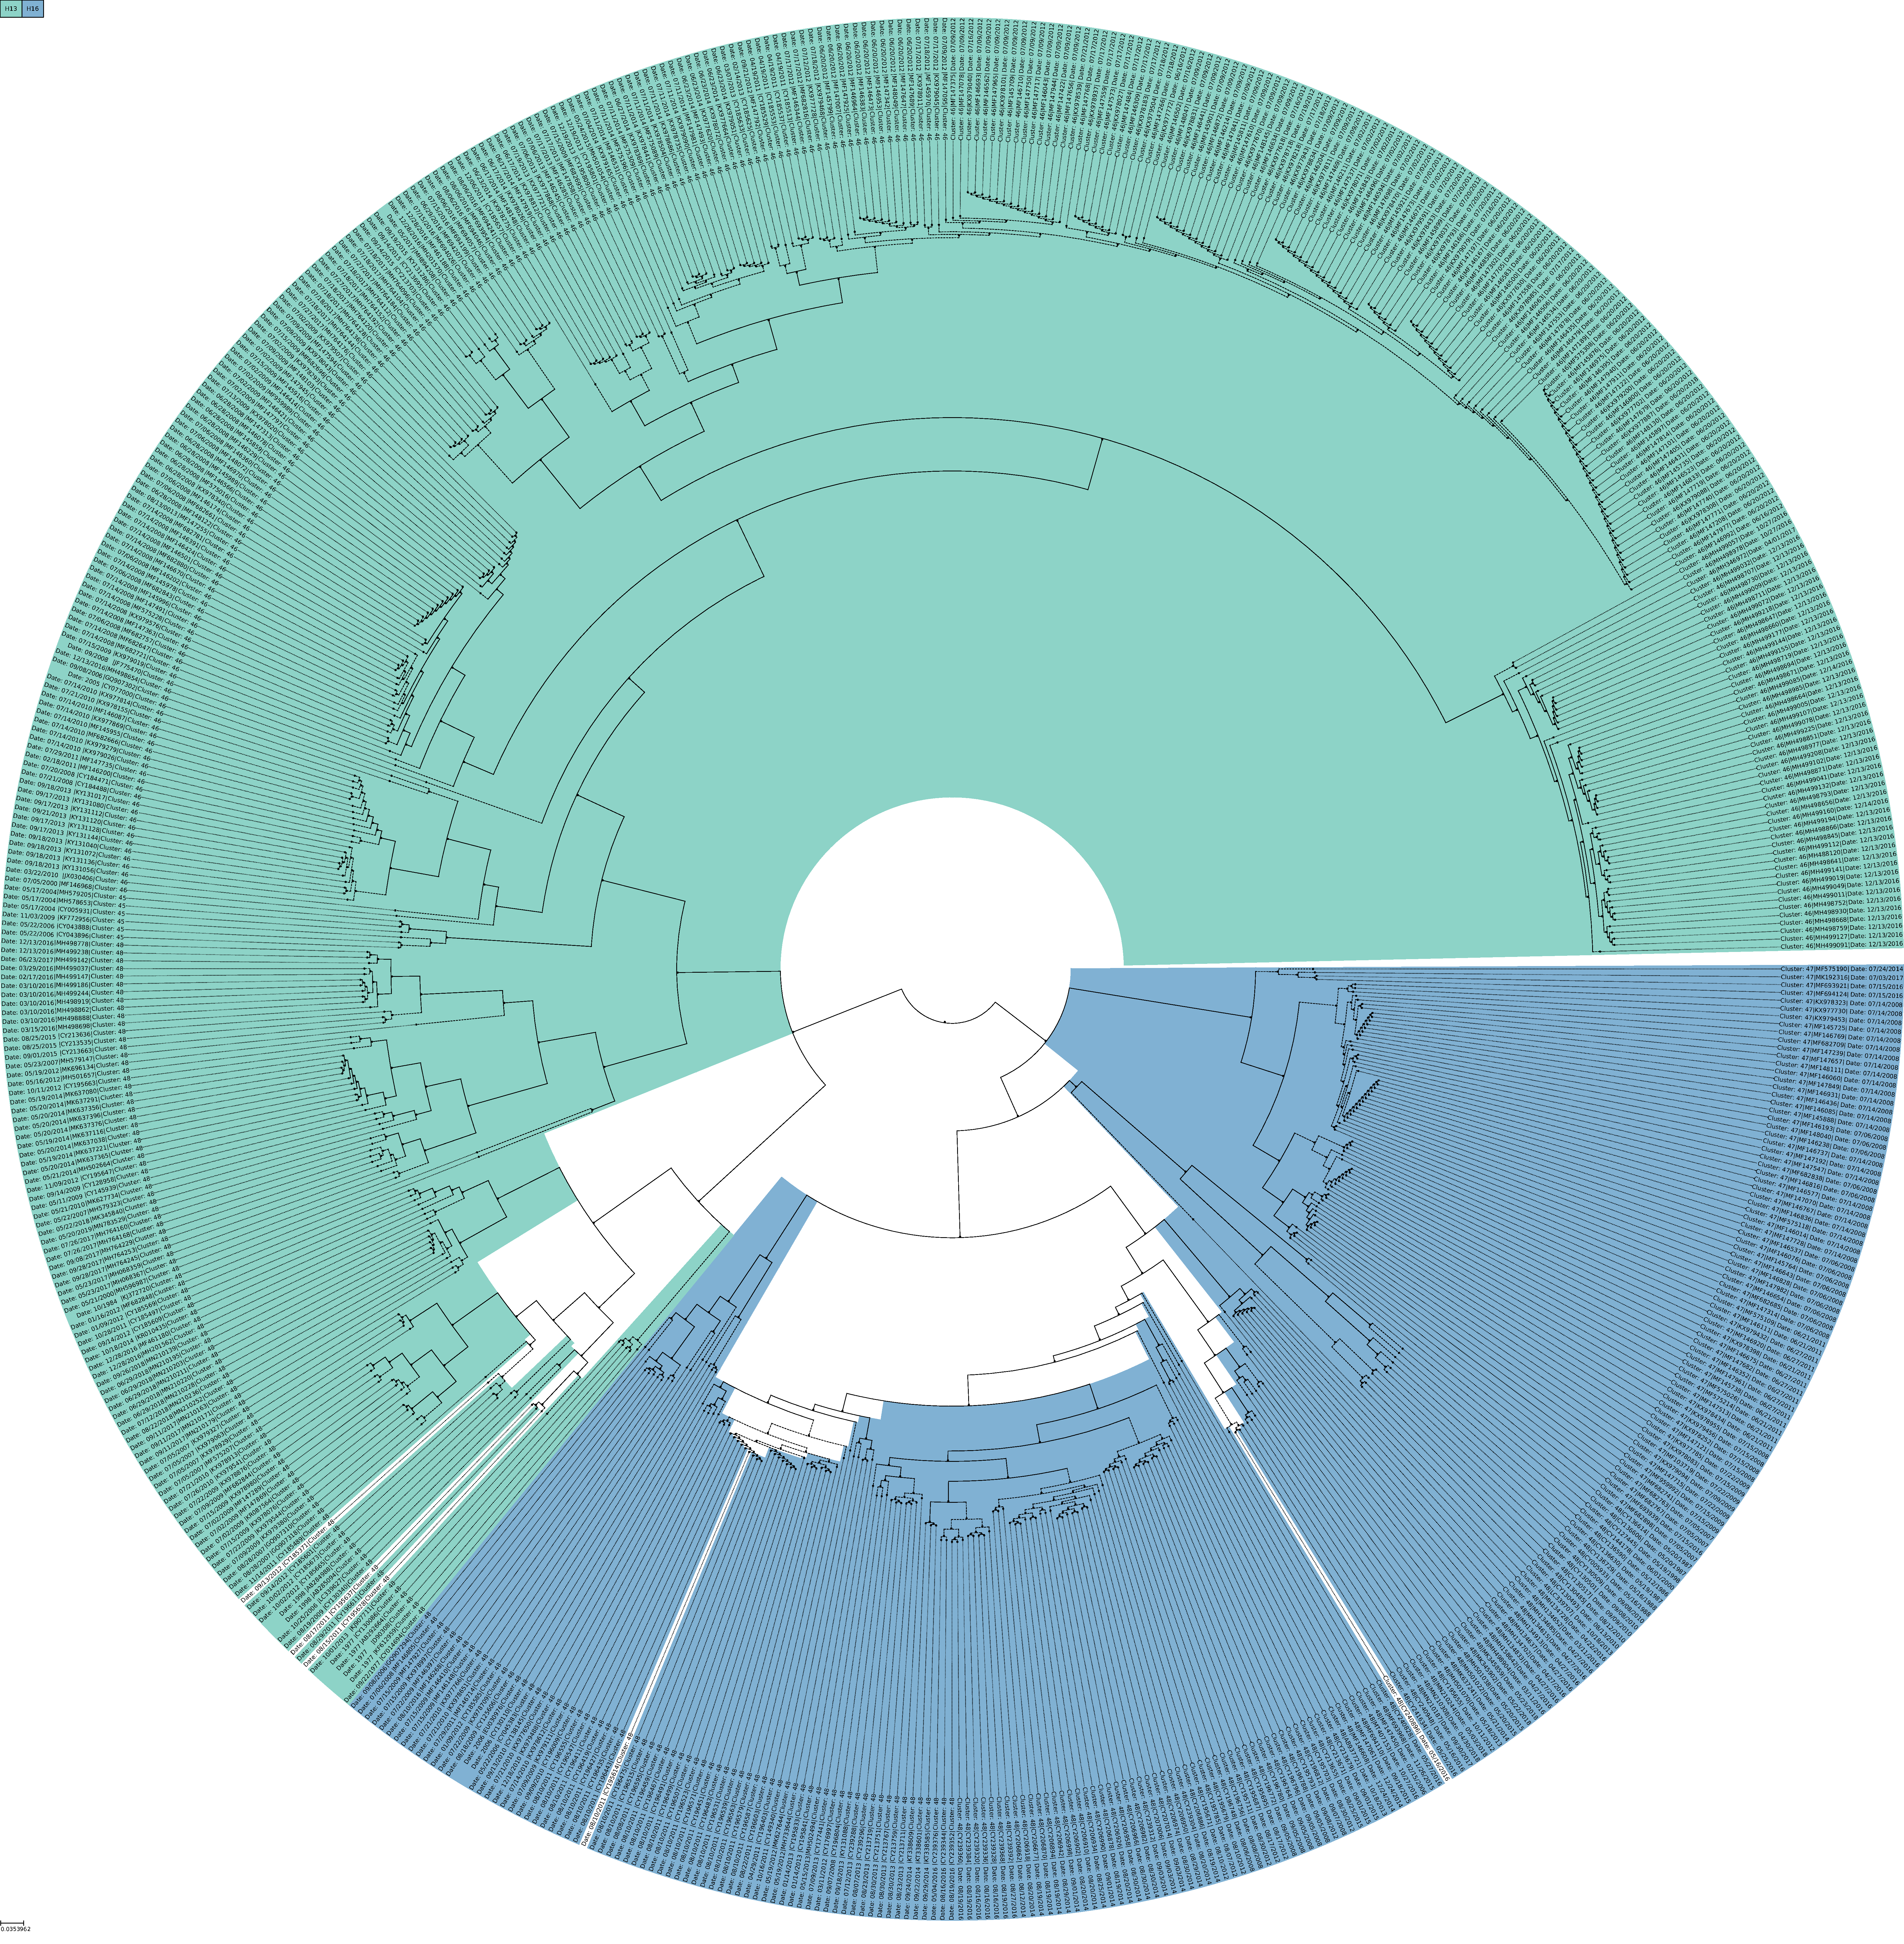
\includegraphics[width=\textwidth]{PCA/Precalculated_Segment_4_H_Cosine.pdf}};
        \begin{scope}[x={(image.south east)},y={(image.north west)}]
            %\draw[help lines,xstep=.1,ystep=.1] (0,0) grid (1,1);
            \draw[draw = none, fill = white] (0,1) rectangle (0.1,0.9);
            \draw[draw = none, fill = white] (0,0) rectangle (0.1,0.1);
            \draw[draw = black, thick, fill = black, fill opacity=0.0] (0.754,0.750) rectangle (0.999,0.505);
            \node at (0.754, 0.505) [fill=Red!80,thick,shape=circle,draw=black,inner sep=2pt] {\textbf{\textsf{C}}};
            %\draw[draw = black, thick, fill = black, fill opacity=0.2] (0.344, 0.603) rectangle (0.589,0.358);
            %\node at (0.344, 0.358) [fill=Red!80,thick,shape=circle,draw=black,inner sep=2pt] {\textbf{\textsf{A}}};
            \node at (0.425,0.525) [arrowstyle=1.5cm, arrowfillR, anchor=east, rotate=270] {\textbf{\textsf{A}}};
            \node at (0.55,0.525) [arrowstyle=1.5cm, arrowfillR, anchor=east, rotate=270] {\textbf{\textsf{B}}};
            %\draw[|-|] (0.975,0.5035) arc[start angle=0,end angle=170,radius=0.475, thick] node[midway,fill=Red!80,thick,shape=circle,draw=black,inner sep=2pt] {\textbf{\textsf{D}}};
            %\node at (0.5,0.505) [shape = circle,inner sep=140pt, fill = black] {};
            \node at (0.31,0.595) [arrowfillG, arrowstyle=1.5cm, anchor=east, rotate=315] {46};
            \node at (0.305,0.51) [arrowfillG, arrowstyle=1.5cm, anchor=east, rotate=45] {45};
            \node at (0.6,0.5) [arrowfillG, arrowstyle=1.5cm, anchor=east, rotate=225] {\rotatebox{180}{47}};
            \node at (0.35,0.455) [arrowfillG, arrowstyle=1.5cm, anchor=east, rotate=90] {48};
            \node at (0.425,0.42) [arrowfillG, arrowstyle=1.5cm, anchor=east, rotate=90] {48};
            \node at (0.54,0.435) [arrowfillG, arrowstyle=1.5cm, anchor=east, rotate=135] {\rotatebox{180}{48}};
        \end{scope}
    \end{tikzpicture}
    \caption[H13/H16 precalculated cosine distance \Acrshort{UPGMA} tree]{\textbf{H13/H16 precalculated cosine distance \Acrshort{UPGMA} tree.} Calculated cosine distance between the k-mer frequency vectors of sequences related to subtype H13 and H16 clusters in \autoref{fig:PCA_Clusteree_Knee_4} were used to build a \gls{UPGMA} tree. The same coloring of the previous tree was used to clarify the difference between H13 and H16 sequences. Uncolored sequences are unclassified ones from the inconclusive cluster 48 and, thereby, not assigned to a single subtype. The numbers in the green arrows indicate the cluster number of the sub trees sequences in \autoref{fig:PCA_Clusteree_Knee_4}. The red arrows are used in the following to point to the trees division into H13 \textbf{\textsf{A}} and H16 \textbf{\textsf{B}}. \autoref{fig:focus} is a enlarged view on the highlighted square at \textbf{\textsf{C}}.}
    \label{fig:Precalculated_Cosine}
\end{figure}

By building a \gls{UPGMA} tree on the non-reduced segment 4 k-mer frequency vectors of the H13 and H16 clusters 45, 46, 47 and 48, the unbiased relation of sequences from these subtypes were analyzed (\autoref{sec:MAFFT}). That way the fundamental use of k-mer frequencies was also validated. Not colored sequences are unclassified sequences (\autoref{fig:Frequency_4}) that also could not be assigned to a subtype, since they were clustered in a inconclusive cluster consisting of H13 and H16. Therefore, these sequences are unclassified sequences from cluster 48 (\autoref{fig:PCA_Clusteree_Knee_4} \textbf{\textsf{B}}).

\begin{figure}[!hbt]
    \centering
    %\begin{adjustbox}{minipage=\dimexpr\textwidth-2\fboxsep-2\fboxrule,fbox}
    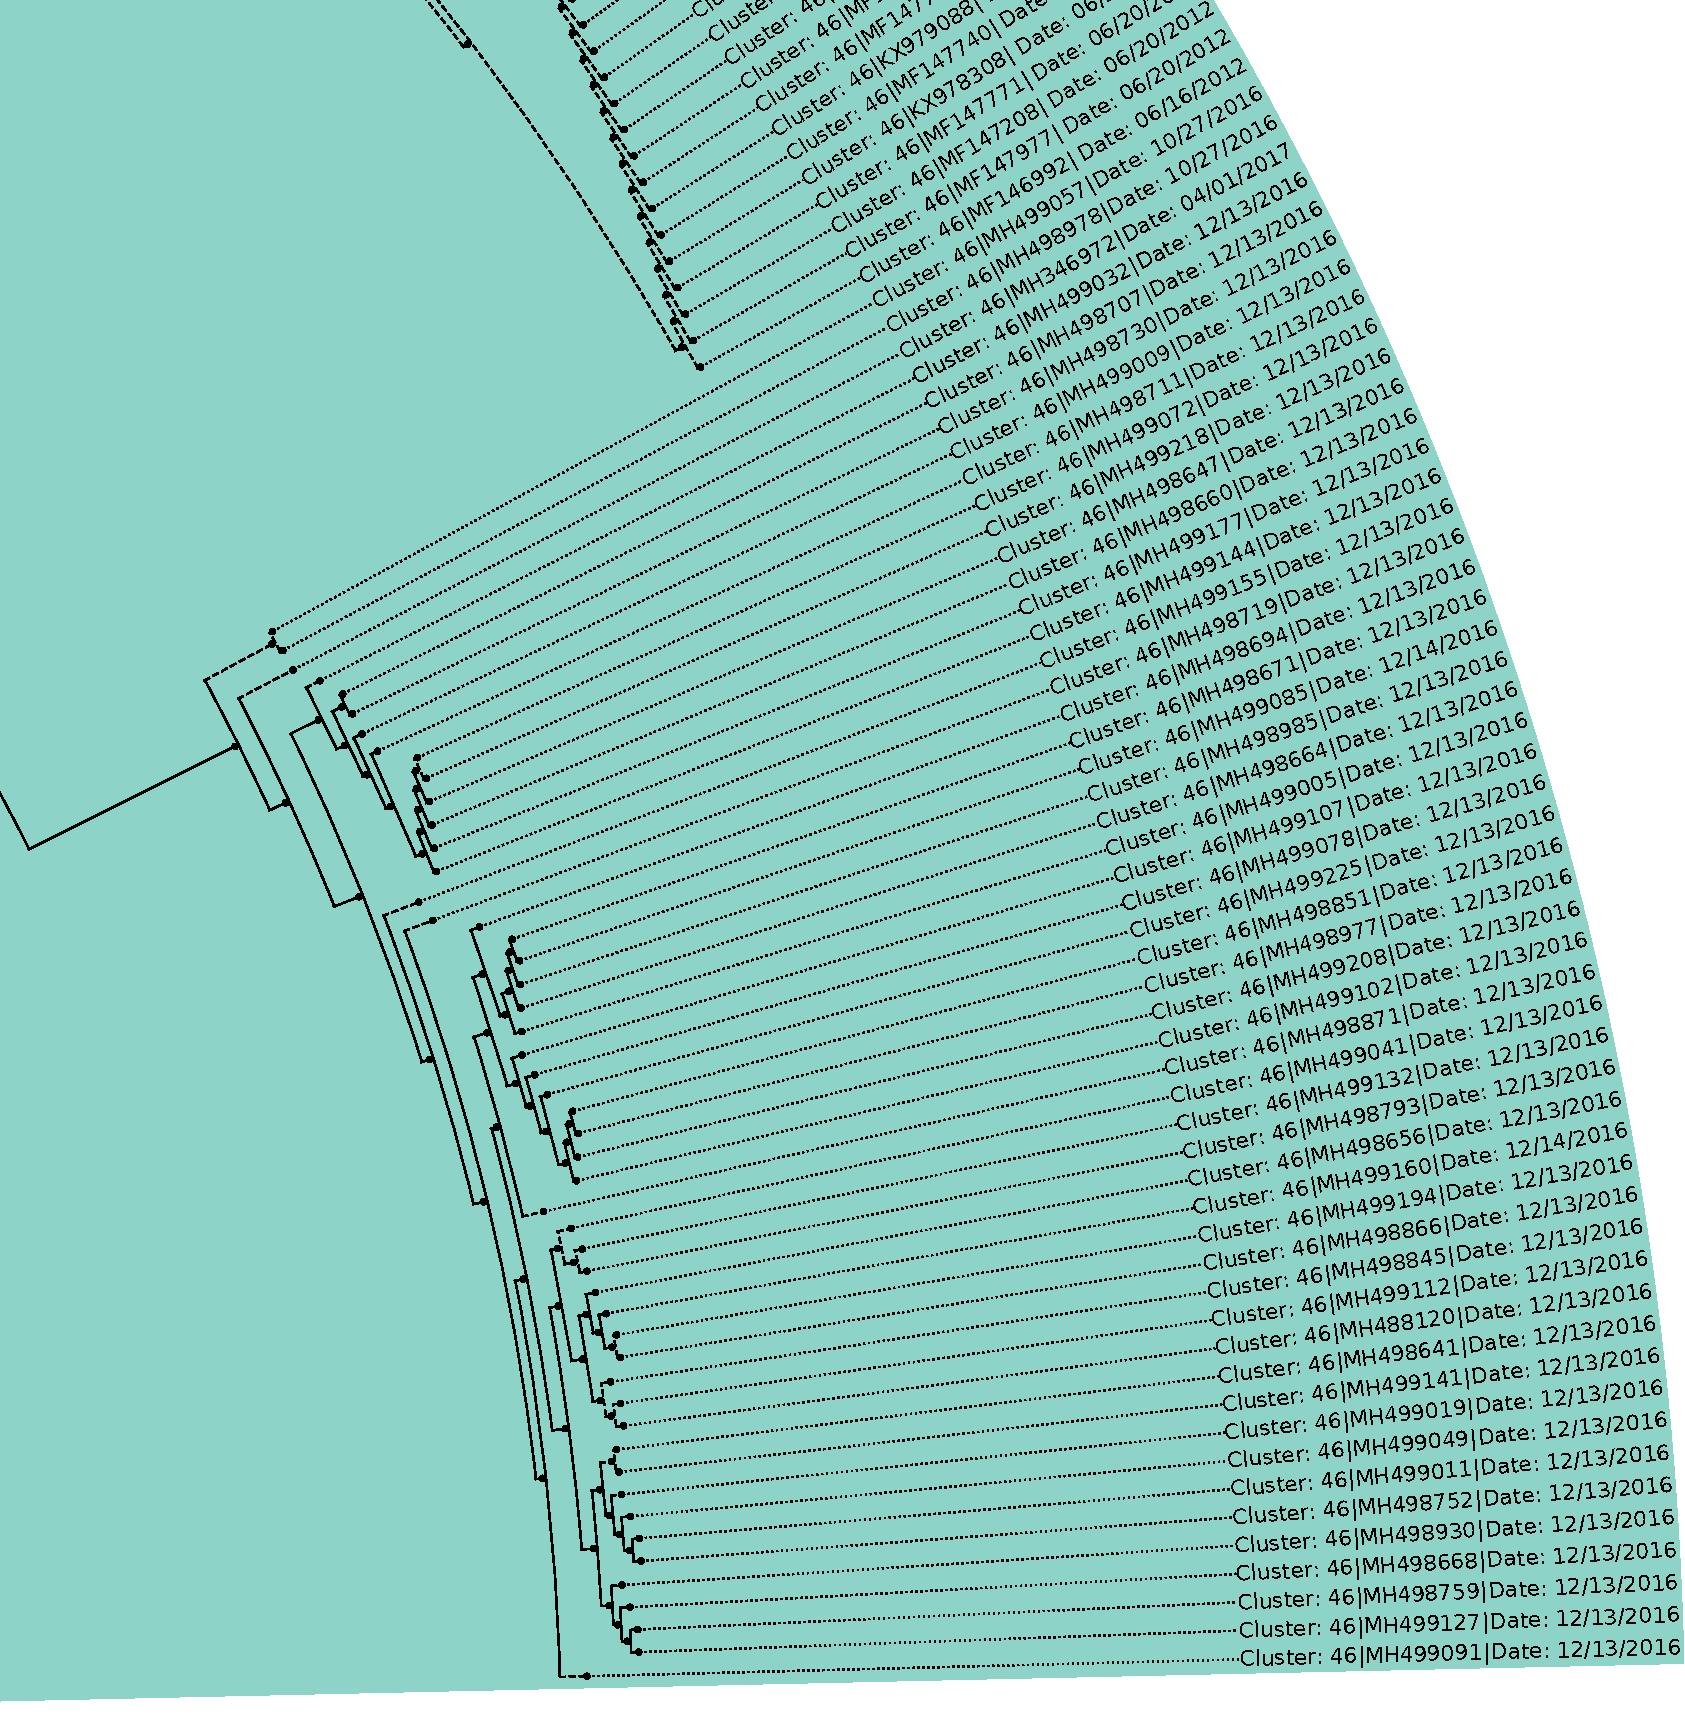
\includegraphics[width=\textwidth]{Graphics/identical.pdf}
    \caption[Relation of collection date and k-mer vector distance]{\textbf{Relation of collection date and k-mer vector distance.} Enlarged view of the by \textbf{\textsf{C}} highlighted square in \autoref{fig:Precalculated_Cosine}. The sequences were labeled according to their collection date to indicate the correlation of the close k-mer frequency vector distance in the tree with their sequences similarity. Labeling with the strain name could misleadingly point in a false direction, since the strain names indicate major difference while the sequences having very high similarity. Thereby the close distance of the vectors of sequences collected on the same date with high sequence similarity point to the precise representation by the k-mer frequency vectors.}
    \label{fig:focus}
\end{figure}

While both subtypes in \autoref{fig:Precalculated_Cosine} are completely separated directly after the trees root, there are also subdivisions for both subtypes directly after. This early subdivision can point to the existence of more subtle variations with major difference to each other than the existing subtype classification reveals. In this case it appears as if at least two subgroups for H13 and at least two or three subgroups for H16 exist. The threshold is difficult to define here and no clustering was performed in this case so this statement is based only on the early subdivision in the k-mer \gls{UPGMA}-tree (\autoref{fig:Precalculated_Cosine} \textbf{\textsf{A}} and \textbf{\textsf{B}}). The exact separation from the root is in line with the centroid guide-tree based on \gls{MSA} were both subtypes are completely separated too (\autoref{fig:PCA_Guidetree_Centroid_4}). Since this is also in line with the subtype classification, the k-mer frequency seems to work for this project. Furthermore, when focusing on a portion of the \gls{UPGMA}-tree with very small difference from sequence to sequence in \autoref{fig:Precalculated_Cosine} \textbf{\textsf{C}}, the similar collection date of all these sequences (12/13/2016) stand out. The only sequences not from this collection date but, nevertheless, included in this sub tree are MH499057, MH498978, MH346972, MH499085, and MH499160. Two of the first three mentioned sequences are from the same collection date but some days prior to the rest, while the third was collected some days after the 12/13/2016. These three sequences are the last linked sequences in the sub tree with the highest distance in comparison to the rest and their collection date is nearly the same as for the rest. The other two sequences with different date MH499085 and MH499160 are in the middle of the sub tree but the collected just one day after the rest. This points in the direction that even small differences are noticed by the k-mer approach. The collection date was used as comparison here because many of the sequences in the sub tree have very different strain names but are almost or completely similar and, thereby, could cause a misinterpretation. MH499085 of strain A/environment/Chile/C20369/2016 and MH498671 of strain A/white\_backed\_stilt/Chile/C20090/2016 differ by their strain names, as the virus was collected apparently completely different but the sequenced genomes are in fact 100\% the same. Around the tree in nearly every case similar collection dates have a small distance based on the k-mer frequency supporting the statement of the usability of k-mer frequencies for \gls{IAV} clustering. Same calculation for the precalculated \gls{UPGMA} tree was also repeated with euclidean distance and can be found in the \autoref{chap:Appendix}.

%frage is hier welche Methode die bessere representation ausstrahlt, sprich UMAP vgl. precalc ja/nein? dann PCA vgl precalc passt? ja/nein?

\section{Ground Truth for Clustering} \label{sec:Comparison_Clustering}

To further investigate in the source of the errors \autoref{fig:PCA_Cluster_Knee_4} \textbf{\textsf{B}} and \textbf{\textsf{D}}, \gls{HDBSCAN} was performed in a more simple manner, without $\varepsilon$ exploration on the small subset of H13 and H16 cluster of segment 4 in \autoref{fig:PCA_Clusteree_Knee_4}. Three different input matrices were used to compare the clustering by \gls{HDBSCAN} and find a ground truth. The first input was the non-reduced set of k-mer frequency vectors used in \autoref{sec:K_mer_Representation} as precalculated matrix with cosine distance (\autoref{sec:MAFFT}). Clustering was then performed and the result visualized as a cluster-tree (\autoref{fig:Simple_Clustertree_Cosine}). 

\begin{figure}[!hbt]
    \centering
    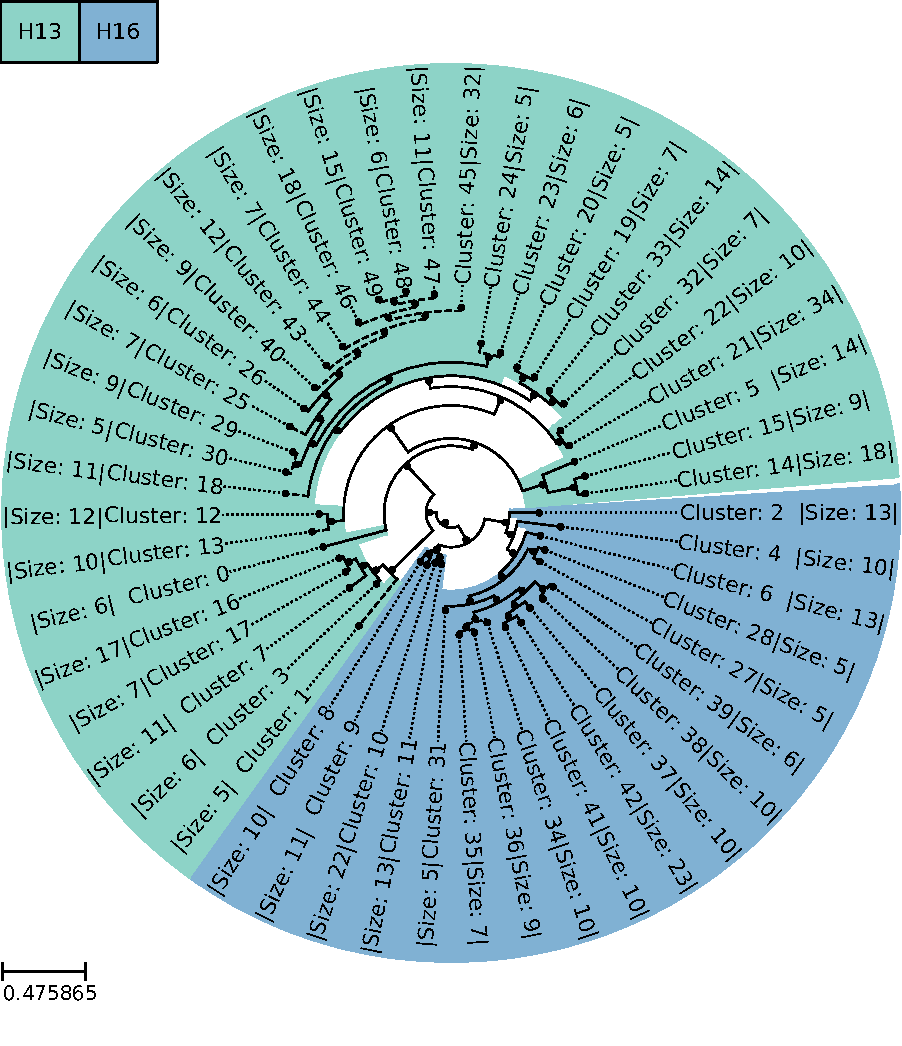
\includegraphics[width=\textwidth]{PCA/Clustertree_Segment_4_H_Cosine.pdf}
    \caption[H13/H16 simple precalculated cosine distance cluster tree]{\textbf{H13/H16 simple cosine distance cluster tree.} Cluster tree, based on the clustering by simple \gls{HDBSCAN} without any $\varepsilon$ exploration and hybrid clustering. The matrix used contained precalculated cosine distances of all the k-mer frequency vectors to each other. The used vectors were calculated from the sequences, present in the H13 and H16 clusters in \autoref{fig:PCA_Clusteree_Knee_4} without reduction with \gls{PCA} or \gls{UMAP}. Therefore, \gls{HDBSCAN} was used with precalculation input instead of a distance metric.}
    \label{fig:Simple_Clustertree_Cosine}
\end{figure}

\begin{figure}[!hbt]
    \centering
    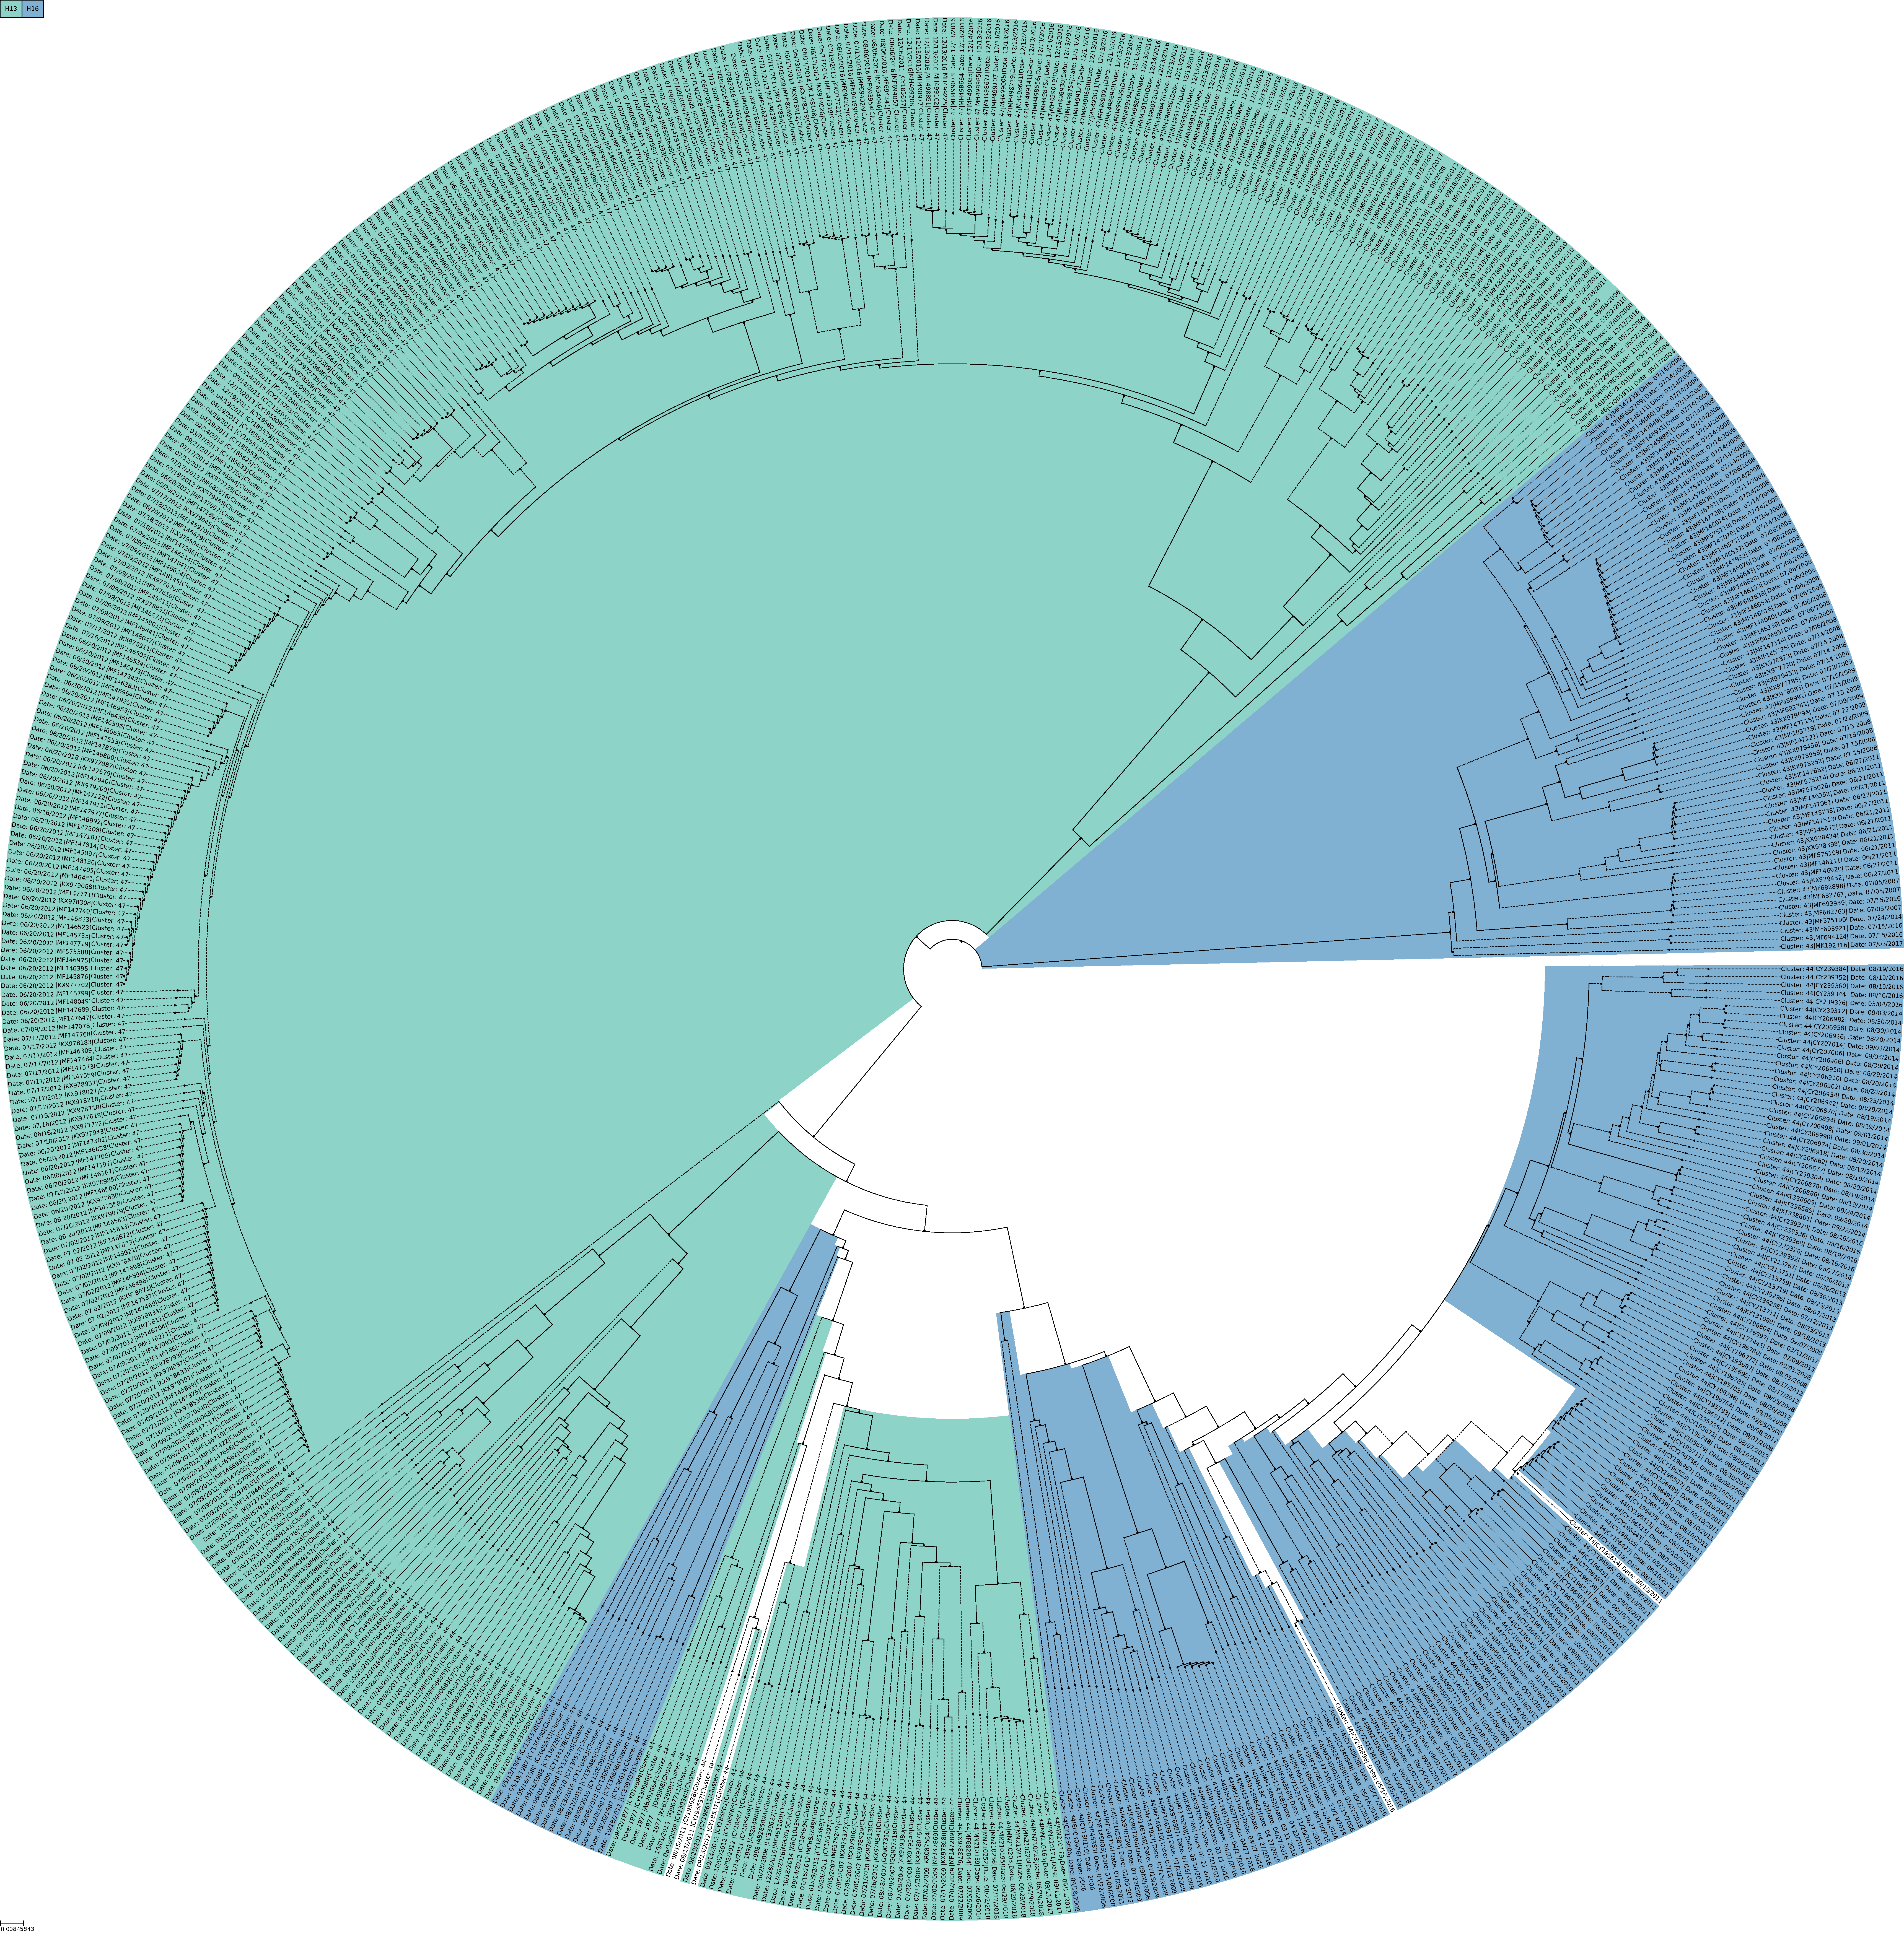
\includegraphics[width=\textwidth]{PCA/Clustertree_Segment_4_H_Focus.pdf}
    \caption[H13/H16 simple precalculated \gls{MSA} distance cluster tree]{\textbf{H13/H16 simple precalculated \gls{MSA} distance cluster tree.} Cluster tree, based on the clustering by simple \gls{HDBSCAN} without any $\varepsilon$ exploration and hybrid clustering. The matrix used contained precalculated \gls{MSA} based distances of all the sequences to each other. The sequences, present in the H13 and H16 clusters in \autoref{fig:PCA_Clusteree_Knee_4} were used for the \gls{MSA}. Therefore, \gls{HDBSCAN} was used with precalculation input instead of a distance metric.}
    \label{fig:Simple_Clustertree_MSA}
\end{figure}

\begin{figure}[!hbt]
    \centering
    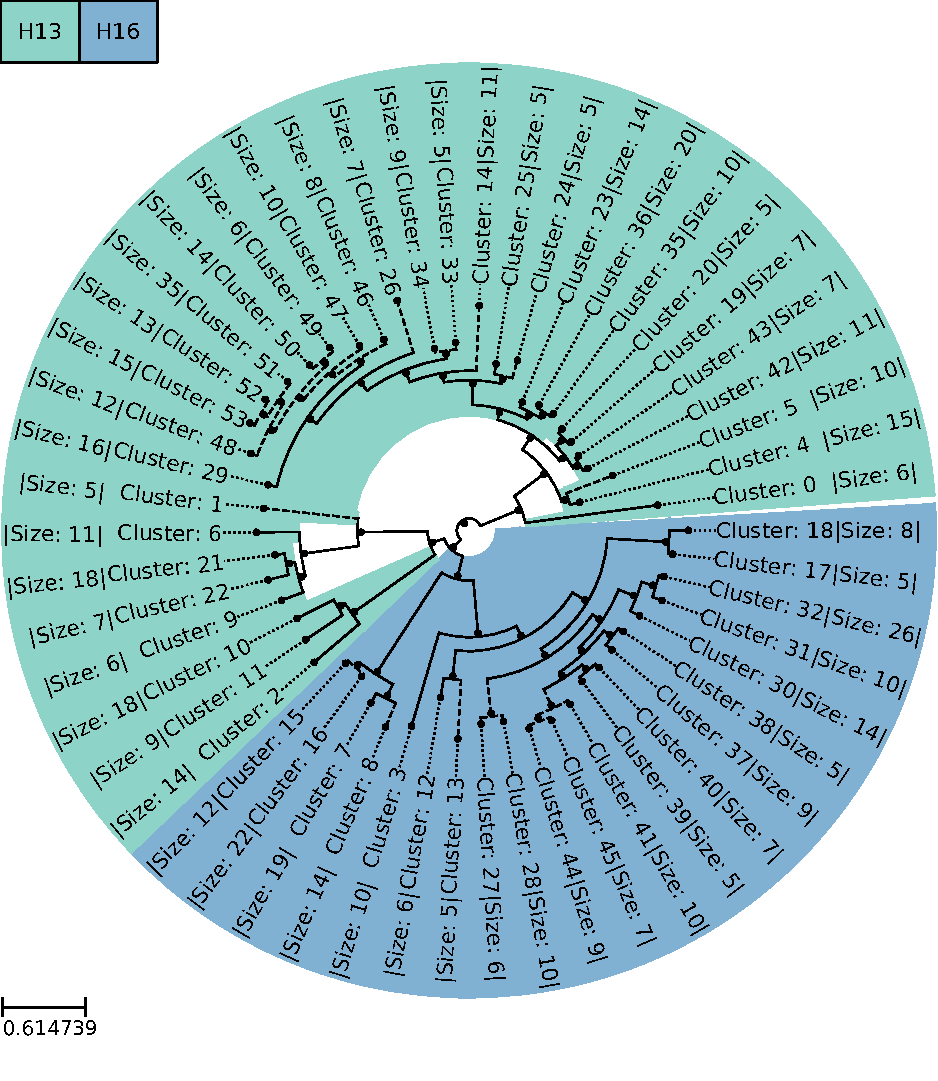
\includegraphics[width=\textwidth]{PCA/Clustertree_Segment_4_H_Simple.pdf}
    \caption[H13/H16 Simple \Acrshort{PCA} vector distance cluster tree]{\textbf{H13/H16 Simple \Acrshort{PCA} vector distance cluster tree.} Cluster tree, based on the clustering by simple \gls{HDBSCAN} without any $\varepsilon$ exploration and hybrid clustering. The used vectors were calculated from the sequences, present in the H13 and H16 clusters in \autoref{fig:PCA_Clusteree_Knee_4} with prior \gls{PCA} reduction to 30 dimensions.}
    \label{fig:Simple_Clustertree_PCA}
\end{figure}

In a similar manner to the precalculated \gls{UPGMA} tree in \autoref{fig:Precalculated_Cosine}, the subtypes are completely separated and split on both sides in two subgroups. This points to the fact, that the \gls{HDBSCAN} clustering of the precalculated cosine distances of the k-mer frequencies are as usable as the k-mer frequencies itself and are able to draw a clear line to separate the subtypes. This finding is in line with the second simple cluster-tree based on the evolutionary distances of a \gls{MSA} containing the same sequences as used in the former precalculated cosine distance clustering (\autoref{fig:Simple_Clustertree_MSA}). The same separation is even more obvious, as the subtypes are farther away from the separation at the trees root. On the side of the H13 sequences, a subdivision is also as clear as the subtype separation. Subgroups in the H16 sequences are, on the other hand, not that clear in \autoref{fig:Simple_Clustertree_MSA}. Maybe the different distances between the subtypes and the subgroups on each side of the subtypes is different because evolutionary aspects like weightings and different costs for nucleotides that are more likely to change are used. In the k-mer frequencies, the pure constellation of nucleotides is used, evolutionary aspects are neglected. Both, the precalculated approach as well as the \gls{MSA} evolutionary distances used the full information available from the sequences themselves, since no reduction with \gls{PCA} was performed. Therefore these cluster trees (\autoref{fig:Simple_Clustertree_Cosine} and \autoref{fig:Simple_Clustertree_MSA}) are the only ground truth for H13/H16 clustering with \gls{HDBSCAN} available. Precalculated clustering with \gls{HDBSCAN} as performed, is a highly computationally expensive task, as with $n$ sequences, the matrices of size $n^2$ have to be calculated and saved to be used in \gls{HDBSCAN}. The calculation is, therefore, not possible without the availability of major RAM space. When using \gls{HDBSCAN} with the k-mer vectors posterior to reduction with \gls{PCA} to 30 dimensions, only a matrix of size $n\times 30$ has to be saved without the necessity of any distance precalculation. To find a clustering method available without using hardware that offers extensive computational power, the simple cluster tree with \gls{PCA} should preferably resemble the previous cluster trees.

Unfortunately, some major differences between the simple cluster tree using \gls{PCA} and the previous precalculated trees using \gls{MSA} and cosine distances occurred (\autoref{fig:Simple_Clustertree_Cosine}, \autoref{fig:Simple_Clustertree_MSA} and \autoref{fig:Simple_Clustertree_PCA}). The same clustering behavior as in the complete cluster tree can be observed as no clear separation on the H13 and H16 clusters is present (\autoref{fig:Simple_Clustertree_PCA} and \autoref{fig:PCA_Clusteree_Knee_4} \textbf{\textsf{B}}). The simple clustering performed with \gls{MSA} distances and precalculated cosine distances showed a clear separation on the subtypes. Since the precalculated distances are solely based on the k-mer frequencies and the \gls{MSA} distances on the evolutionary aspect and both methods present a clear separation, the \gls{PCA} or dimension reduction step seems to be the origin of the clustering error in \autoref{fig:PCA_Cluster_Knee_4} \textbf{\textsf{B}} and \textbf{\textsf{D}}. 

As already mentioned the precalculated cluster trees use the whole available amount of information given by the sequences, either by direct use of the nucleotide comparisons with \gls{MSA} (\autoref{fig:Simple_Clustertree_MSA}) or by using the k-mer frequency vectors without reducing the dimension (\autoref{fig:Simple_Clustertree_Cosine}). Thus, the amount of information remaining in the vectors did not seem to suffice for the given task. The simple clustering was also performed with the same subset of H13 and H16 sequences reduced with \gls{UMAP} posterior to \gls{PCA} as described in \autoref{sec:Clustering} and can be found in the \autoref{chap:Appendix}. A third precalculated cluster tree using euclidean distance instead of cosine distance, offering a similar result to the one using cosine distance is also present there.

\section{Differences in dimension reduction} \label{sec:Dimension_Reduction}

To investigate the processing behavior prior to the clustering and, thereby, find explanations for the mentioned errors, the small H13 and H16 subset of segment 4 $k$-mer frequencies, were reduced by \texttt{PCA} and \texttt{UMAP} to two components for in detail visualization. Comparison to \texttt{UMAP} was done although the method was already declared as not appropriate, to validate this statement again and see the impact of different neighbor values. 

\vspace{1em}

The target of the reduction prior to the \texttt{HDBSCAN} clustering, was to find a representation of the data that is most suitable to be used for the clustering, by preserving the information with a lower complexity. As explained in \autoref{sec:K_mer_Representation} and \autoref{sec:Comparison_Clustering} the optimal representation of the vectors should make a clear difference between H13 and H16 and is, thereby, also used as the ground truth in the following. Since the vectors are visualized in two dimensions, the term point instead of vector is used.

\begin{figure}[!hbt]
    \centering
    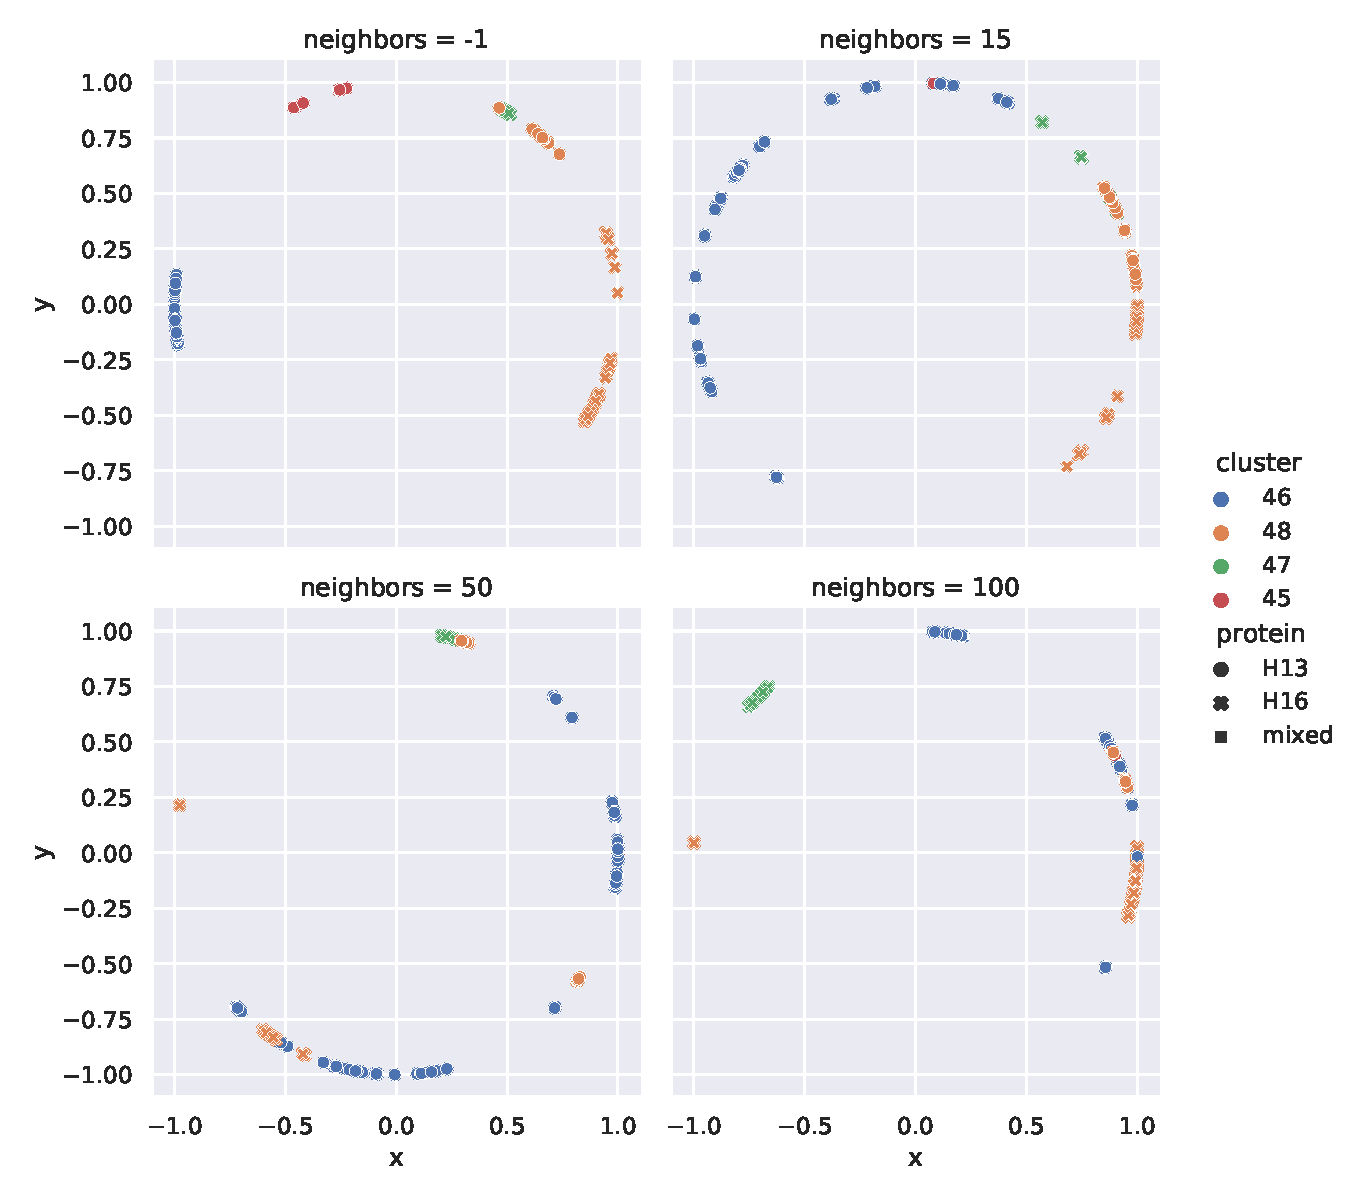
\includegraphics[width=\textwidth]{PCA/Difference_Segment_4_H_metric_cosine.pdf}
    \caption[Comparison of H13/H16 component reductions]{\textbf{Comparison of H13/H16 component reductions.} The subset of sequences from the H13 and H16 clusters in \autoref{fig:PCA_Clusteree_Knee_4} were reduced down to two dimensions enabling simple visualization. Cluster labeling was performed according to \autoref{fig:PCA_Clusteree_Knee_4}. Sole use of \texttt{PCA} (top left picture) as well as the combination with \texttt{UMAP} (other three pictures) was performed as described in \autoref{sec:Dimension_Reduction} with the reduction to two components for visualization. For the combination of \texttt{PCA} and \texttt{UMAP} different values for the neighbors setting were used, the \texttt{UMAP} standard value 15, a average value 50 and the standard value of this project 100. The subtype of the sequences were labeled by different types of points.}
    \label{fig:Reduction_Comparison}
\end{figure}

\vspace{1em}

The visualization of the reduction by \texttt{PCA} is denoted as neighbors value -1 (\autoref{fig:Reduction_Comparison}). It shows five different accumulations of points. Labeling of these points is based on the original clustering example in \autoref{fig:PCA_Cluster_Knee_4}. This is becoming apparent when focusing on the cluster 48 points containing H13 and H16 sequences. That way a fundamental distribution on the points of H13 and H16 can be reviewed as well. 

%When using the right side as possible indication for clustering, all the points and accumulations of points are very close to each other. Nonetheless a separation with a imagined clustering can be made very easy by building two clusters of the blue points, one of the red and green and three of the orange points. Still, all the points related to H13 would be merged with the orange ones of H16 before the orange H16 points would be merged with the green ones of H16. Thereby the difference between H13 and H16, the higher-ranking goal would be not accomplished because the orange points are so close to each other. 
\newpage

The reduction with \texttt{PCA} on the subset results in easy separable accumulations of the cluster 46 and 48 points in \autoref{fig:Reduction_Comparison} (neighbors = -1). The distribution of these points is basically in line with the result shown in \autoref{fig:PCA_Cluster_Knee_4}, as their accumulations are well separated, building the two clusters with the same sequences in both figures. The major difference, however, is the distance between the accumulations of cluster 48 points to each other as well as to the ones of cluster 47. This would probably result in a imaginary clustering of unchanged cluster 46 and 45 and two or three clusters consisting of the cluster 48 points of which one also contains the points of cluster 47. It seems as if the distance of the cluster 47 points and the H13 cluster 48 points is largely affected by the reduction. The difference between cluster 46 and 45 in the \autoref{fig:Reduction_Comparison} (neighbors = -1) picture is on the other hand preserved and would result in clustering similar to \autoref{fig:PCA_Cluster_Knee_4}. In \autoref{fig:PCA_Cluster_Knee_4} cluster 47 and 48 are also relatively close related as they would be linked on the next higher tree-node.

\vspace{1em}

In \autoref{fig:Reduction_Comparison} (neighbors = -1) it appears as if the points of cluster 47 and 48 are possibly quite similar, which is not the case as the \autoref{fig:Precalculated_Cosine} subtrees clearly show the wanted separation of H13 and H16 in cluster 48 as well as the wanted distance to 47. Keeping the lower complexity in mind, the consequence of lowering the dimension by \texttt{PCA} to two dimension seems to preserve most of the information related to the difference of cluster 45 and 46. The difference of the subtype separation inside 48 as well as the overall difference to 47 seems on the other hand to be lost completely and cause the unwanted effects. Since the ground truth separation of \autoref{fig:Precalculated_Cosine} seems to be partially present in \autoref{fig:PCA_Cluster_Knee_4}, by at least separating 47 completely from 48, the higher number of dimensions might be in direct connection to the correct separation of some part of H13 and H16. Therefore, the number of components should be increased to the maximum of 50, that still preserves all functions of \texttt{HDBSCAN} for spanning-tree building. 

\vspace{1em}

Comparing these results to the use of \texttt{UMAP} with different settings of the neighbors value, the impact of this parameter becomes clear. The higher the value, the more crowded the points. This also explains the crowded behavior in \autoref{subfig:Normalisation_UMAP}. Since a neighbors value of 100 was used as standard in this project, the values are overall crowded in groups of at least 100 points. The random subset for \autoref{subfig:Normalisation_UMAP} was reduced by the same setting with \texttt{UMAP} despite the small sample size used there. The small random sample in addition to a high neighbors value resulted in a low number of overall distribution to clarify this behavior. Aside from the example in \autoref{subfig:Normalisation_UMAP} the usage of a high neighbors value through the project was well reasoned and based on the huge size of the dataset used as described in \autoref{sec:Dimension_Reduction}. The same value as well as 15 and 50 neighbors was used on the subset of H13 and H16 segment 4 sequences to visualize the difference. 

\vspace{1em}

None of the settings results in a separation as good as with the sole use of \texttt{PCA}. With the \texttt{UMAP} standard neighbors value of 15 all the points are next to each other and there is no reasonable cluster building possible \autoref{fig:Reduction_Comparison} (neighbors = 15). Furthermore, H13 points would be merged with H16 points before merging with others from H13, thereby breaking the subtype division similar to the \texttt{PCA} use. Aside from the fact that the other points, when using \texttt{PCA}, are well separated. Setting the neighbors value to 50 results in a spreading of the cluster 46 points and mixing with little islands of cluster 48 points \autoref{fig:Reduction_Comparison} (neighbors = 50). With a neighbors value of 100 a separation into imaginary clusters is possible, when ignoring the cluster labeling and only taking the subtypes labeling into consideration. This is, therefore, the only setting with use of \texttt{UMAP} that would provide a more of less reasonable separation of the subtypes in imaginary clusters. However, clusters of different subtypes are closer than to similar subtypes, resulting also in no real subtype separation, even when ignoring the cluster 47 points that might be very sensible to the magnitude of preserved information.

%With normalization and without some information seem to be missing necessary to separate the orange points and the green ones. While on the left side the distance was underestimated to an extend making the orange H13 points and the green H16 points collide, the distance on the right side is overestimated, making the subtype distance of the H13 and H16 orange points to small. Since the separation between red and blue, as well as H13 orange and H16 orange is clearer, the method using normalization is still proved to be the better one, in the circumstances that the location of the green points is caused by the low dimension which is proved by \autoref{fig:PCA_Cluster_Knee_4} showing a separation between 47 and 48 and the right method not producing any better results related to the green points. 
\vspace{1em}

In conclusion, the use of PCA gives the best results compared the ones with \texttt{UMAP}. Still there are challenges to overcome as could be seen with the position of the cluster 47 points. Maybe increasing the information preserved by the \texttt{PCA} would give clearer results as assumed. This project aimed to find high-quality representations of \gls{IAV} genomes for the purpose or clustering in a extend that was never reached before. Therefore, the usability of hybrid \texttt{HDBSCAN} with parameters as good as possible was of higher importance than the use of \texttt{UMAP} at all costs. In the results of the project \texttt{PCA} performed better than \texttt{UMAP} but only with all the tested parameters. Thus, it might be possible to find parameters for \texttt{UMAP} not explored in this project to represent the genomes even better in a equal low-dimension in the future. Also, change of \texttt{UMAP} in favor of \texttt{t-SNE} could be tested in terms of vector representation quality.

\section{The New proposed Classification} \label{sec:Serotype_Classification}

\blindtext

%neue classification vorschlagen blablabla
% vielleicht bisschen evolution black sea gull etc

\begin{figure}[!hbt]
    \centering
    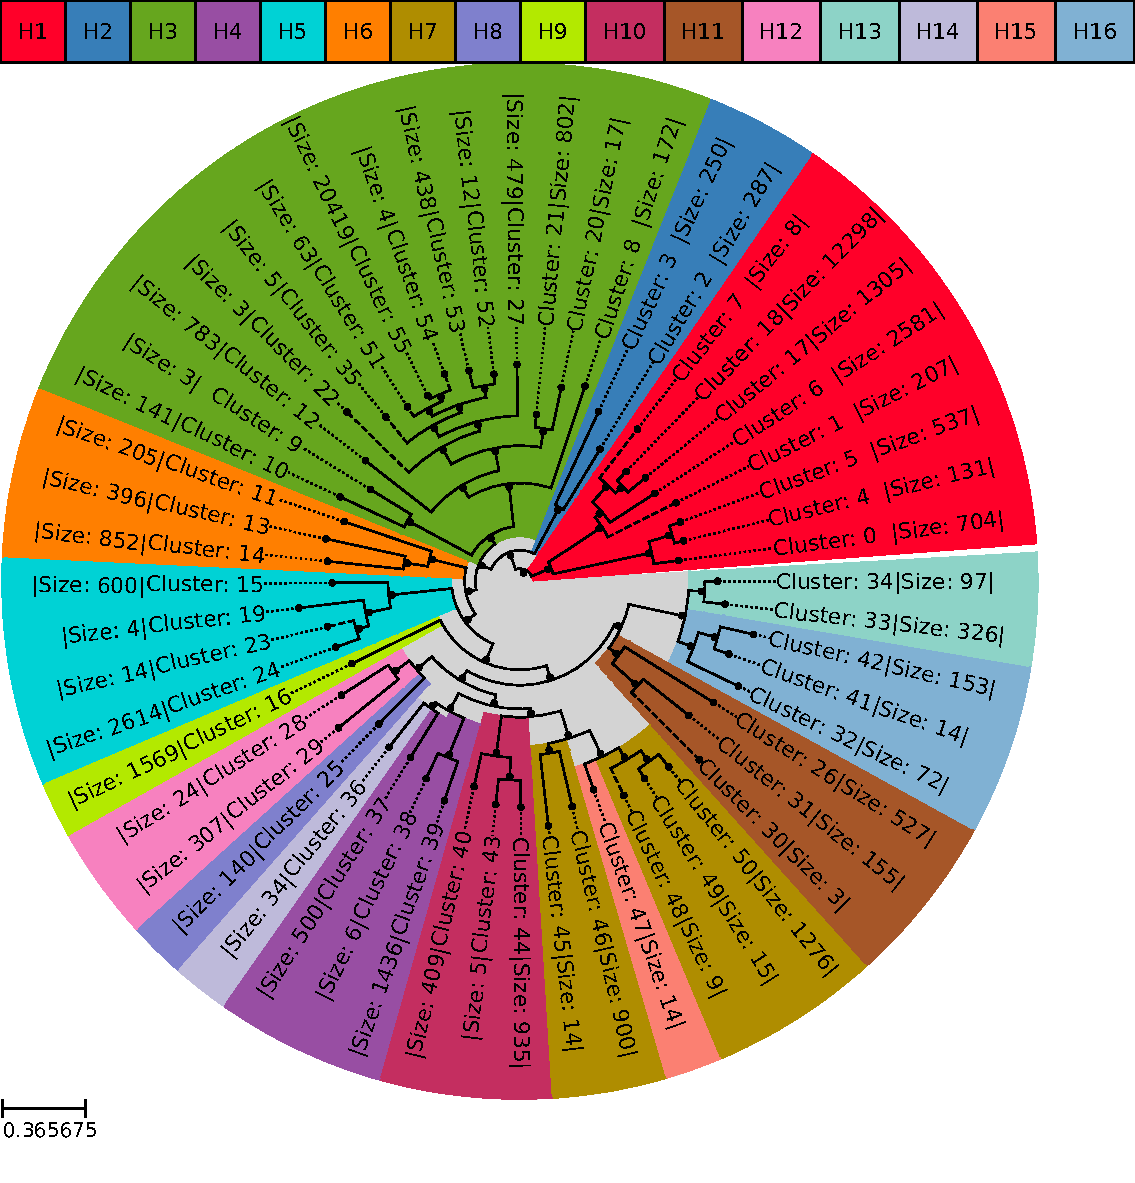
\includegraphics[width=\textwidth, draft]{Results/Clustertree_Segment_4.pdf}
    \caption[Final Segment 4 Clustertree (\Acrshort{PCA})]{\textbf{Final Segment 4 Clustertree (\Acrshort{PCA}).} .}
    %\label{fig:PCA_Clusteree_Final}
\end{figure}